% =====================================================================
%  Cluster analysis of CART-synthesised data (formerly "Downstream utility
%  of synthetic data for clustering")
%  Journal of Classification submission draft -- v5.
%  v5 implements the co-authors' decisions on the proposal report
%  (J. Cortes, D. Fernandez): fixed candidate range {2,...,8} as primary,
%  bootstrap null (B = 30) for count agreement and geometric metrics,
%  scale-free metrics, appendices moved to the supplementary material.
%  See CHANGES_v5.md. Sentences in V. Lopez's Conclusions paragraph that
%  were changed are marked with "% VL-EDIT" for her approval.
%
%  Every number in this file comes from results/fullrange_summary.json,
%  results/bootstrap_summary.json or results/v5_extra_numbers.json; the
%  tables in tables/*.tex are generated by src/synthclust/v5_tables.py.
%
%  TEMPLATE
%  --------
%  This compiles against Springer Nature's sn-jnl.cls (v3.x), which is in this
%  folder together with sn-basic.bst.
%
%  sn-jnl.cls and sn-basic.bst are Springer Nature's official copies, from the
%  journal article template package (December 2024 version) on Springer's LaTeX
%  author-support page (replaced 27 Oct 2026; the earlier third-party copies are
%  in _backup_v5_preDJ/class_thirdparty/).
%
%  \pdfmapfile below is a workaround for a broken font-map index on the build
%  machine. On a normal TeX installation, delete that one line.
%
%  BUILD VARIANTS (see joc_prep/README.md; ./build_submission.sh does this)
%  ---------------------------------------------------------------------
%  Two switches, set before this file is read:
%    \def\SetReferee{}     JoC referee layout: 12 pt, double-spaced, single
%                          column, A4 with 30 mm margins (joc_prep/joc_referee)
%    \def\SetBlind{true}   anonymised build (joc_prep/blind.tex): author block,
%                          repository URL and identifying clauses removed,
%                          PDF metadata emptied
%  e.g. pdflatex -jobname=main_blind '\def\SetReferee{}\def\SetBlind{true}% =====================================================================
%  Cluster analysis of CART-synthesised data (formerly "Downstream utility
%  of synthetic data for clustering")
%  Journal of Classification submission draft -- v5.
%  v5 implements the co-authors' decisions on the proposal report
%  (J. Cortes, D. Fernandez): fixed candidate range {2,...,8} as primary,
%  bootstrap null (B = 30) for count agreement and geometric metrics,
%  scale-free metrics, appendices moved to the supplementary material.
%  See CHANGES_v5.md. Sentences in V. Lopez's Conclusions paragraph that
%  were changed are marked with "% VL-EDIT" for her approval.
%
%  Every number in this file comes from results/fullrange_summary.json,
%  results/bootstrap_summary.json or results/v5_extra_numbers.json; the
%  tables in tables/*.tex are generated by src/synthclust/v5_tables.py.
%
%  TEMPLATE
%  --------
%  This compiles against Springer Nature's sn-jnl.cls (v3.x), which is in this
%  folder together with sn-basic.bst.
%
%  IMPORTANT: sn-jnl.cls here was obtained from a third-party GitHub mirror
%  because Springer's own download page was unreachable from the machine this
%  was built on. Before submitting, replace it with the official copy from
%  Springer's LaTeX author-support page (or open the template on Overleaf and
%  download the zip) and rebuild. The document body should not need changes.
%
%  \pdfmapfile below is a workaround for a broken font-map index on the build
%  machine. On a normal TeX installation, delete that one line.
% =====================================================================
\documentclass[pdflatex,sn-basic]{sn-jnl}

\pdfmapfile{=local.map}          %% build-machine workaround; delete elsewhere

%%%% Standard Springer Nature preamble (from sn-article.tex)
\usepackage{graphicx}%
\usepackage{multirow}%
\usepackage{amsmath,amssymb,amsfonts}%
\usepackage{amsthm}%
\usepackage{mathrsfs}%
\usepackage[title]{appendix}%
\usepackage{xcolor}%
\usepackage{textcomp}%
\usepackage{manyfoot}%
\usepackage{booktabs}%

% Indicator function (review round 2: \mathbb{1} rendered as a stray glyph).
\newcommand{\ind}{\mathbf{1}}
% Vectors and matrices in bold (JoC: vectors and matrices must be
% distinguishable from scalars).
\newcommand{\bx}{\mathbf{x}}
\newcommand{\bX}{\mathbf{X}}
\newcommand{\bmu}{\boldsymbol{\mu}}
\newcommand{\bg}{\mathbf{g}}
\newcommand{\bR}{\mathbf{R}}

\begin{document}

\title{Cluster Analysis of CART-Synthesised Data: A Factorial Simulation of
       $k$-Means and Ward's Linkage}

\author[1]{Oriol Farr\'es Vilar}
\author[2]{Jordi Cort\'es}
\author[3]{Xinnuo Chen}
\author[4]{Victoria L\'opez}
\author[2]{Daniel Fern\'andez}

\affil[1]{Department of Computer Science,
          Universitat Polit\`ecnica de Catalunya, Barcelona, Spain}
\affil[2]{Department of Statistics and Operations Research,
          Universitat Polit\`ecnica de Catalunya, Barcelona, Spain}
\affil[3]{Department of Statistical Science,
          University College London, London, United Kingdom}
\affil[4]{CUNEF Universidad, Madrid, Spain}

\abstract{Synthetic data replace confidential records, so their value depends
on whether analyses of the release reproduce the original ones. We study
this for cluster analysis in a factorial simulation of 144 scenarios crossing
separation, number of groups, dimensionality, correlation and distribution
family (720{,}000 evaluations), applying $k$-means and Ward's linkage to data
synthesised by sequential CART. Agreement between the numbers of groups
estimated from synthetic and original data rises with separation. $k$-means
reproduces the original number more often than Ward ($0.84$ versus $0.81$),
on skewed Gamma data ($0.81$ versus $0.73$) but not on Normal data ($0.87$
versus $0.89$). A bootstrap null shows that this reflects the greater
stability of the $k$-means estimate under resampling, not smaller damage from
CART. Resampling alone also reproduces most centroid and dispersion distortion.
Utility should be judged against a resampling reference.}

\keywords{Synthetic data, CART synthesis, \texttt{synthpop}, $k$-means, Ward's
          linkage, Number of clusters, Cluster stability, Bootstrap null}

\maketitle

% =====================================================================
\section{Introduction}
% =====================================================================

Synthetic data are artificial records produced by a generative model fitted to
a confidential dataset, released in place of the original records so that the
statistical structure of the data is retained while no real individual is
exposed. The idea originates in statistical disclosure control, where
\citet{rubin1993} proposed treating the confidential values as missing and
releasing multiply-imputed replacements, and \citet{little1993} developed the
companion analysis of masked data; \citet{drechsler2011} gives a book-length
treatment of the resulting framework, and \citet{matthews2011} survey the wider
family of disclosure-limitation methods within which synthesis sits. Synthetic
data were initially developed mainly for statistical agencies, but their
application has since expanded to many other fields. General-purpose
synthesisers are now distributed as statistical software
\citep{nowok2016,templ2017}, and administrative-data research is an active
area of application \citep{kokosi2022}. Synthetic records are also generated
for health services research \citep{gonzales2023,giuffre2023}, for
biobehavioural science, where they additionally serve reproducibility and
hypothesis generation \citep{quintana2020}, and, increasingly, through deep
generative architectures applied to tabular data \citep{goyal2024,zhao2024}.

Synthetic data are mainly generated to support subsequent analyses, and cluster
analysis is one of the most widely used unsupervised approaches: given
unlabelled observations, it partitions them into groups that are internally
homogeneous and mutually distinct. Two main approaches have dominated applied
practice for decades: centroid-based methods, such as $k$-means
\citep{macqueen1967,steinley2006}, which minimise the within-cluster sum of
squares and remain the most widely deployed clustering algorithms
\citep{ahmed2020}; and agglomerative hierarchical methods, such as Ward's
linkage \citep{ward1963}, which build a dendrogram by successive merging and
do not require the number of groups to be fixed in advance. Both remain
central to contemporary applications: in single-cell transcriptomics, where
partitions define cell types \citep{zappia2018}, and in mass cytometry, where
the choice among clustering methods materially changes the biological
conclusion \citep{liu2019}.

These two areas intersect whenever a clustering analysis must be performed on
data that cannot be released in raw form. In clinical and administrative
settings, for example, subgroup discovery can be highly valuable, but access
to the original data is often restricted for privacy reasons
\citep{goncalves2020,elemam2020,bhanot2021}. In model development, access to
the original data can also be slow or limited, and synthetic records then
serve as an augmentation and development resource \citep{rankin2020}.
Synthetic data can therefore provide a practical solution in both situations.
However, when an analysis is performed on synthetic rather than original data,
it is important to assess whether the resulting partition is similar to the
one that would have been obtained from the original records. This is what the
\emph{analytical utility} of synthetic data refers to.

Analytical utility can be assessed from a general and from a specific
perspective. \emph{General} utility asks whether the synthetic data resemble
the original in a global sense, and \emph{specific} utility asks whether a
particular analysis yields matching conclusions \citep{snoke2018}. The
distinction matters because the two can diverge: a generator that reproduces
marginal distributions and low-order correlations faithfully may still distort
the higher-order geometry on which a specific procedure depends. Empirical work
bears this out. Benchmarking studies of synthetic health records find that
utility rankings depend heavily on which downstream task is used to measure
them \citep{yan2022,elemam2022}, and direct replications of published analyses
on synthetic counterparts show agreement that varies by study and by estimand
\citep{reinerbenaim2020}. A recent systematic review of tabular synthesis tools
makes the same point from the measurement side, finding no consensus on which
utility metrics should be reported and little agreement between them
\citep{lautrup2024}. Utility is therefore not a scalar property of a dataset;
it is a property of the pairing between a dataset and the analysis applied to
it.

Clustering provides a useful approach for assessing this relationship. Unlike
a regression coefficient, which summarises a conditional mean and is
comparatively robust to local perturbation, a partition is sensitive to the
fine structure of the point cloud: relative positions, local density,
separability and within-group dispersion. Two datasets can share identical
means, variances and pairwise correlations and still yield entirely different
partitions. Distortion that a generator introduces into local geometry may
therefore appear in a clustering analysis before it appears in a resemblance
check.

This article asks whether CART-based sequential synthesis, the default
non-parametric engine of \texttt{synthpop} \citep{nowok2016} and a widely used
method for tabular data, preserves the structure that clustering relies on.
This study extends the line of inquiry opened by \citet{chen2025}, which
established a simulation harness for this question but restricted attention to
$k$-means on Normal data and relied on a resemblance statistic that proved
insensitive to structural quality. We broaden the scope in three directions: a
second clustering method, Ward's linkage, which shares the within-cluster
sum-of-squares criterion of $k$-means but optimises it by greedy agglomeration;
a skewed distribution family that exposes the axis-aligned behaviour of
tree-based synthesis; and a set of structural metrics that compare the
partition recovered from the synthetic data with the partition recovered from
the original data.

Whether a synthetic dataset leads the analyst to the same number of clusters
as the original is a question about the stability of cluster analysis under
perturbation, a topic with an extensive resampling literature
\citep{benhur2002,dudoit2002,tibshirani2005,hennig2007,luxburg2010}. We use
that literature to calibrate our agreement measure: the reference point is not
perfect agreement but the agreement obtained when the synthetic data are
replaced by a bootstrap resample of the original.

The utility of synthetic data for clustering analysis is assessed through three
main objectives. First, to determine whether CART-synthesised data preserve the
structure needed to recover the number of clusters, and how this depends on
separation, number of groups, dimensionality, feature correlation and
distribution family. Second, to determine whether the cluster structure is
preserved beyond the number of clusters: how much fidelity of centroid
location, within-group dispersion and group sizes is lost under synthesis, and
which design factors drive that loss. Third, to determine whether partitioning
and hierarchical methods respond similarly to synthetic distortion, or whether
one is systematically more robust than the other. We address these questions
with a factorial simulation. For each scenario, several original datasets are
simulated from a mixture with known group structure, and each original dataset
is then synthesised many times with CART. We compare the number of clusters
recovered from each synthetic dataset with two references: the true number of
groups used to simulate the original dataset, and the number of clusters
recovered from that original dataset by the same algorithm. Each synthetic
result is also set against the same quantity computed on bootstrap resamples
of the original dataset, which separates the effect of CART from ordinary
resampling variability.

% =====================================================================
\section{Methods}
% =====================================================================

The study is a controlled factorial simulation. We first define the data and
the discrepancy being studied and the two clustering algorithms, then the
generation of original and synthetic data, then the metrics used to quantify
structural degradation and their bootstrap reference, and finally the way
those metrics are summarised across replications.

\subsection{Data and discrepancy}

Each original dataset is an $N \times p$ data matrix
$\bX_R = (\bx_1,\dots,\bx_N)^{\top}$ of $N$ observations on $p$ continuous
variables, with rows $\bx_i \in \mathbb{R}^p$ and columns (variables)
$X_1,\dots,X_p$, together with a vector of planted group labels
$\bg = (g_1,\dots,g_N)^{\top}$, $g_i \in \{1,\dots,k\}$, which is known by
construction but is never used by the clustering algorithms. A generative
mechanism $G$ produces a synthetic $N \times p$ matrix $\bX_S = G(\bX_R)$ with
the same variables. Let $A$ be the downstream algorithm, producing summaries
$\theta_R = A(\bX_R)$ and $\theta_S = A(\bX_S)$. We study the discrepancy
\begin{equation}
  \Delta(\theta_R, \theta_S) = f(N, p, \rho, \sigma, k, F),
  \label{eq:discrepancy}
\end{equation}
as a function of the sample size $N$, dimensionality $p$, feature
correlation $\rho$, separation $\sigma$, number of latent groups $k$ and
distribution family $F$. A generator is useful for a task over a region of the
design space when $\Delta$ remains small throughout it, and the content of an
evaluation is the shape of $\Delta$: which factors inflate it, which leave it
unchanged, and whether different algorithms respond similarly.

In the clustering setting, $\theta$ comprises the estimated number of groups
$\hat{k}$ together with the geometry of the recovered partition: its
centroids, its group sizes and its within-group dispersion. Accordingly
$\Delta$ is instantiated as a family of structural-fidelity measures defined in
Section~\ref{sec:metrics}.

To study how synthesis affects cluster structure, we use simulations with
known ground truth rather than real administrative data. Each scenario fixes a
configuration $(N, p, k, \rho, \sigma, F)$ for which the true group membership
of every point is known by construction. This makes it possible to separate the
difficulty of the clustering problem itself from the distortion introduced by
synthesis, avoids relying solely on resemblance-based evaluations, and allows
$\Delta$ in Eq.~\eqref{eq:discrepancy} to be traced as an explicit function of
each design factor.

\subsection{Clustering algorithms}
\label{sec:algorithms}

We compare two standard approaches: $k$-means \citep{macqueen1967} as a
partitioning method, and agglomerative clustering with Ward's linkage
\citep{ward1963} as a hierarchical method. $k$-means minimises the
within-cluster sum of squares and so tends to favour convex, isotropic groups
of comparable size \citep{steinley2006,xiong2009}, with decision boundaries
given by the bisectors of the centroid Voronoi tessellation; we retain the
lowest-inertia solution over ten initialisations. Ward's linkage merges, at
each step, the pair of clusters whose union least increases the total
within-cluster error sum of squares. The two methods therefore share a
variance-based criterion and differ in how they optimise it: Ward's merges are
greedy and never revisited, so a merge driven by a local density irregularity
early in the hierarchy propagates to the final partition, whereas $k$-means
reassigns points iteratively. Because synthesis perturbs exactly such local
irregularities, the two optimisation strategies may respond differently to it.
Classical comparisons found that the sensitivity of clustering methods to
error perturbation differs between methods and between types of perturbation,
and that the behaviour of $k$-means depends on its starting configuration
\citep{milligan1980}. Both objectives are stated formally in Section~S7 of the
supplementary material.

\subsection{Data generation}

\subsubsection{Original data}

Each original matrix $\bX_R$ contains $N = 1000$ observations drawn from a
$k$-component mixture in $\mathbb{R}^p$ with known group labels and equal
component sizes ($N/k$ observations each, up to rounding). The minimum pairwise
centroid distance is controlled by the separation $\sigma$: the first centroid
$\bmu_1$ sits at the origin and each subsequent centroid $\bmu_j$ is drawn
uniformly on the sphere of radius $\sigma$ about the origin and accepted only
if it lies at distance at least $\sigma$ from all centroids already placed.
The centroids are drawn afresh for every original dataset. Within-component
covariance equals the $p \times p$ correlation matrix $\bR$ with unit diagonal
and off-diagonal entries $\rho$, giving uncorrelated (spherical) components at
$\rho = 0$ and correlated (elliptical) components at $\rho = 0.4$; separation
is therefore expressed in units of the within-component standard deviation. In
the \emph{Normal} family, components are multivariate Gaussian with mean
$\bmu_j$ and covariance $\bR$. In the \emph{Gamma} family, independent Gamma
variates (shape $=1.5$, rate $=5$) are standardised to zero mean and unit
variance within each component, correlated using the Cholesky factor of $\bR$
\citep[chap.~4]{johnson1987}, and shifted to the component centroid. The two
families thus share their first two moments within components and differ only
in shape: before correlation is induced, each Gamma margin has skewness
$2/\sqrt{1.5} \approx 1.63$, producing right-skewed groups that stress the
axis-aligned nature of CART.

The factors we vary are the same high-level geometric properties used to
parameterise cluster-analysis benchmarks generally, namely overlap between
groups, their number, the ambient dimension and the shape of the components
\citep{qiu2006,zellinger2025}; here they serve not to benchmark clustering
algorithms against each other but to locate the regions in which synthesis
preserves the structure those algorithms depend on.

Table~\ref{tab:design} lists the design factors. Each factor is varied to
examine how it affects the conditions under which synthesis succeeds or fails:
crossing all five gives $3 \times 4 \times 3 \times 2 \times 2 = 144$
scenarios. For each scenario, $n = 5$ independent original datasets are
simulated, and each original dataset is synthesised $m = 1000$ times, resulting
in $144 \times 5 \times 1000 = 720{,}000$ synthetic-versus-original
evaluations.

\begin{table}[t]
\centering
\caption{Factors of the simulation design and the question each addresses.
         Crossing all five gives 144 scenarios; with $n=5$ independent original
         datasets per scenario and $m=1000$ synthetic datasets generated from
         each, the design yields 720{,}000 evaluations.}
\label{tab:design}
\small
\begin{tabular}{llp{6.2cm}}
\toprule
Factor & Levels & Rationale \\
\midrule
Separation $\sigma$      & $0.1,\,2,\,6,\,10$ & Spans overlapping to clearly
  distinct groups; tests how much separation between groups is needed before
  synthesis can preserve the structure. \\
Number of groups $k$     & $2,\,3,\,4$        & More groups increase the
  complexity of the cluster structure that the generator needs to
  preserve. \\
Dimensionality $p$       & $2,\,5,\,10$       & Each synthesised dimension
  compounds the axis-aligned leaf structure of the generator. \\
Correlation $\rho$       & $0,\,0.4$          & Tests whether dependence
  between features degrades a variable-by-variable synthesis. \\
Distribution family $F$  & Normal, Gamma      & Contrasts symmetric Gaussian
  density with skewed Gamma density. \\
\midrule
Sample size $N$          & $1000$ (fixed)     & Held constant so that
  variation is attributable to the factors above. \\
\bottomrule
\end{tabular}
\end{table}

\paragraph{Expected directions.} The rationales in Table~\ref{tab:design}
imply the following expected directions, which the analysis examines. Both
agreement measures should increase with separation $\sigma$. Recovery of the
planted number of groups should decrease with $k$. Geometric distortion should
increase with $p$, because each synthesised coordinate adds its own leaf
structure. Correlated components ($\rho = 0.4$) should be harder for a
variable-by-variable synthesiser than uncorrelated ones, and skewed Gamma
components harder than Normal ones. For the comparison between the two
algorithms no direction was fixed in advance: they share a criterion and
differ in how they optimise it (Section~\ref{sec:algorithms}).

\subsubsection{Synthetic data (CART)}
\label{sec:cart}

For every original dataset, synthetic data $\bX_S = G(\bX_R)$ are generated
with the CART engine of \texttt{synthpop} \citep{nowok2016}, using proper
synthesis (the trees are fitted to a bootstrap sample of the original data)
and a minimum leaf size of ten. Variables are synthesised sequentially in the
order $X_1,\dots,X_p$. The first variable is sampled from its observed marginal
distribution. Each subsequent variable $X_j$ is then modelled by a regression
tree \citep[chap.~8]{breiman1984} on the already-synthesised variables, and
synthetic values are drawn from the empirical distribution of the observed
values in the corresponding leaf,
\begin{equation}
  X_j^{\text{syn}} \sim
    \widehat{P}\bigl(X_j \mid
      \text{leaf}(X_1^{\text{syn}},\dots,X_{j-1}^{\text{syn}})\bigr).
  \label{eq:cart}
\end{equation}

This makes the method flexible and distribution-free, but it imposes an
axis-aligned, piecewise-constant structure on the joint distribution: the
synthetic point cloud is assembled from rectangular blocks whose boundaries are
the tree splits, and synthetic values are resampled observed values. When the
original data are smooth and symmetric, these blocks tile the space finely
enough to be barely visible; when the data are skewed or heavy-tailed, they can
become visible as a hardening of smooth density gradients into discrete steps.
Detecting this failure mode, and measuring how strongly it propagates into the
recovered partition, is the purpose of the evaluation. The group label is
appended as the last variable of the synthesis sequence, so it does not
influence the synthesis of the features; it is never used by the clustering
algorithms.

\paragraph{Software and seeds.} Original data were generated and synthesised
under \textsf{R} 4.3 \citep{rcore2024} with \texttt{synthpop} 1.9.2
\citep{nowok2016}, \texttt{mvtnorm} 1.4.2 and \texttt{arrow} 25.0.0; the
\texttt{rpart} version of that run was not recorded, and the synthetic draws
were reproduced bit for bit with \texttt{rpart} 4.1.24 under \textsf{R} 4.3.3.
Clustering and evaluation used Python 3.12 with \texttt{scikit-learn} 1.9.0
\citep{pedregosa2011}, \texttt{numpy} 2.5.1, \texttt{scipy} 1.18.0,
\texttt{pandas} 3.0.5 and \texttt{pyarrow} 25.0.0. All seeds derive from a
base seed of 16. The 144 scenarios are shuffled after \texttt{set.seed(16)},
one seed per scenario is then drawn after a second \texttt{set.seed(16)}, and
the five replicates of a scenario are generated in turn from that seed. The
synthetic draw $m$ of replicate $r$ uses the seed
$16 + 10^{7}g + 10^{5}r + m$, where $g$ is the position of the scenario in the
list of original file names sorted by \textsf{R}; because \textsf{R}'s
\texttt{sort()} is locale-dependent, this index, and hence the synthetic data,
is reproduced only under the \texttt{en\_US.UTF-8} collation (the C collation
gives a different index), and the distributed per-scenario seed table records
$g$ explicitly. Every $k$-means fit, on original and synthetic data alike, uses
\texttt{random\_state = 42} with ten initialisations, so the original and
synthetic fits share their starting points. Both stages are embarrassingly
parallel over scenarios and were distributed across $18$ worker processes on a
single multi-core workstation (Section~S8 of the supplementary material).

\subsection{Evaluation metrics}
\label{sec:metrics}

Structural utility is quantified by two count-agreement measures and three
geometric-fidelity measures, each set against a bootstrap reference
(Section~\ref{sec:null}). All variables are standardised before clustering.
The scaler is fit on the original data and applied unchanged to the
corresponding synthetic dataset, so that all geometric quantities are
expressed in a common coordinate system; standardising each dataset separately
would rescale away part of the very distortion the metrics are meant to detect
(see Section~\ref{sec:limitations}).

\paragraph{Number of groups.}
For a dataset and an algorithm, the number of groups is estimated by maximising
the average silhouette width \citep{rousseeuw1987} over the fixed candidate
range $\{2,\dots,8\}$, applied identically to original and synthetic data.
Earlier work \citep{chen2025} used the range $\{2,\dots,\min(k+3,8)\}$, which
ties the search to the planted $k$; the count analyses under that range are
reported as a sensitivity analysis in Section~S3 of the supplementary material.
We write $\hat{k}_R$ for the estimate obtained from an original dataset and
$\hat{k}_{S,m}$ for the estimate obtained from the $m$-th synthetic dataset
generated from it, and $\hat{k}_{R,m}$ for the estimate from the original
dataset that generated synthetic dataset $m$. For a configuration with $M$
evaluations we report two agreement proportions,
\begin{equation}
  \mathrm{RR} = \frac{1}{M} \sum_{m=1}^{M}
    \ind\bigl[\hat{k}_{S,m} = k\bigr],
  \qquad
  \mathrm{AG} = \frac{1}{M} \sum_{m=1}^{M}
    \ind\bigl[\hat{k}_{S,m} = \hat{k}_{R,m}\bigr],
  \label{eq:sr}
\end{equation}
where $\ind[\cdot]$ is the indicator function. The recovery rate $\mathrm{RR}$
compares the synthetic estimate with the planted number of groups. It
therefore confounds two sources of failure: distortion introduced by
synthesis, and the inability of the clustering procedure to recover the
planted structure even from the original data (for instance, when the groups
overlap so strongly that a single diffuse cloud is a reasonable description).
The agreement $\mathrm{AG}$ compares the synthetic estimate with the estimate
from the original data, obtained with the same algorithm and the same
selection rule, and so removes the first source. It does not remove a third:
$\hat{k}$ varies from sample to sample even without synthesis, so part of any
disagreement is ordinary sampling instability of the silhouette estimate.
$\mathrm{AG}$ is therefore read against the bootstrap null
$\mathrm{AG}_0$ of Section~\ref{sec:null}. $\mathrm{RR}$, together with the
recovery rate of the original data itself, $\ind[\hat{k}_R = k]$, is reported
to separate the sources of failure.

\paragraph{Geometric fidelity.}
The geometric metrics are computed with the number of clusters fixed at the
planted $k$ on both sides, so that they describe the geometry of the
partition conditional on the correct count. They require the groups recovered
from $\bX_S$ to be matched to those from $\bX_R$, since cluster labels are
arbitrary. We build the matrix of pairwise centroid distances between the $k$
original and $k$ synthetic clusters and solve the resulting linear assignment
problem \citep{kuhn1955}, obtaining the one-to-one matching that minimises
total centroid distance. All fidelity metrics are computed on the aligned
clusters.

\paragraph{Group-balance error ($\Delta G$).}
This metric evaluates whether the distribution of observations across clusters
is preserved under synthesis. It is defined as
\begin{equation}
  \Delta G = \bigl| G_S - G_R \bigr|,
  \label{eq:dgini}
\end{equation}
where $G_R$ and $G_S$ are the Gini coefficients of the cluster-size vectors of
the partitions recovered from the original and synthetic data. For sizes
$\{n_1,\dots,n_k\}$,
\begin{equation}
  G = \frac{\sum_{a=1}^{k}\sum_{b=1}^{k} |n_a - n_b|}
           {2k \sum_{a=1}^{k} n_a},
  \label{eq:gini}
\end{equation}
with $G = 0$ for perfectly equal groups. A value of $\Delta G$ close to $0$
indicates that synthesis has preserved the distribution of cluster sizes.
Because the planted groups have equal sizes, $G_R$ reflects only the imbalance
that the algorithm itself produces on the original data.

\paragraph{Mean centroid distance (MCD).}
This metric measures the average distance between the centroids of the
original clusters and the centroids of the corresponding synthetic clusters.
With aligned original and synthetic centroids $\bmu_j^R$ and $\bmu_j^S$,
\begin{equation}
  \mathrm{MCD} = \frac{1}{k} \sum_{j=1}^{k}
    \bigl\lVert \bmu_j^R - \bmu_j^S \bigr\rVert ,
  \label{eq:mcd}
\end{equation}
so small values indicate that synthesis preserves the location of the groups.

\paragraph{Mean variance difference (MVD).}
This metric evaluates whether the synthetic clusters retain a dispersion
similar to that of the original clusters. Writing $v_j^R$ and $v_j^S$ for the
mean squared distance of points to their centroid in aligned original and
synthetic clusters,
\begin{equation}
  \mathrm{MVD} = \frac{1}{k} \sum_{j=1}^{k} \bigl| v_j^R - v_j^S \bigr| .
  \label{eq:mvd}
\end{equation}

\paragraph{Scale-free versions.}
Both MCD and MVD are expressed in the units of the scaler, which is fit on the
pooled original data; because the spread of the pooled data grows with the
separation between groups, a standardised unit corresponds to a larger
within-component distance at large $\sigma$. We therefore also report two
scale-free versions. The relative variance difference
\begin{equation}
  \mathrm{RVD} = \frac{1}{k} \sum_{j=1}^{k}
    \Bigl| \frac{v_j^S}{v_j^R} - 1 \Bigr|
  \label{eq:rvd}
\end{equation}
is the average relative error of the within-cluster dispersion, and
$\mathrm{MCD}_{\mathrm{sd}} = \mathrm{MCD}/s_w$ expresses the centroid
displacement in units of the within-component standard deviation
$s_w = \{\sum_{i} \lVert \bx_i - \bmu_{g_i} \rVert^2 / (Np)\}^{1/2}$ of the
original dataset in the scaled coordinates, where $\bmu_{g_i}$ is the mean of
the planted group of observation $i$. We also report $\mathrm{MVD}/p$, since
$v_j$ is a sum over the $p$ coordinates.

\subsection{Bootstrap null}
\label{sec:null}

Proper synthesis in \texttt{synthpop} first draws a bootstrap sample of the
original data and then fits the CART models to it. A bootstrap resample of the
original data is therefore the synthesis procedure without the tree step, and
it is the natural reference for how much disagreement ordinary resampling
alone produces. For each of the 720 original datasets we draw $B = 30$
bootstrap resamples of its $N$ rows, apply the scaler fitted on the original
data unchanged, and run the same silhouette scan, giving estimates
$\hat{k}_{b}$, $b = 1,\dots,B$. The bootstrap agreement
\begin{equation}
  \mathrm{AG}_0 = \frac{1}{B} \sum_{b=1}^{B}
    \ind\bigl[\hat{k}_{b} = \hat{k}_{R}\bigr]
  \label{eq:ag0}
\end{equation}
is averaged over datasets in the same way as $\mathrm{AG}$, and each method is
compared with its own null through the excess $\mathrm{AG} - \mathrm{AG}_0$: a
negative excess means that synthesis loses agreement beyond what resampling
already loses. The same resamples give a \emph{geometric floor} for every
fidelity metric: MCD, MVD, $\Delta G$, RVD and $\mathrm{MCD}_{\mathrm{sd}}$
computed, at the planted $k$, between the partition of the original data and
the partition of the bootstrap resample, averaged over the $B$ resamples. The
excess of an observed metric over its floor is the part of the distortion
attributable to CART beyond resampling. Resample $b$ of original dataset $r$
in scenario $s$ is drawn with the \texttt{numpy} generator seeded by
$(20260929, s, r, b)$, and the same resample is used for both algorithms, so
that the comparison between methods is paired. With $B = 30$, the Monte Carlo
standard error of a scenario-level $\mathrm{AG}_0$ is at most about $0.04$.

\subsection{Statistical analysis}
\label{sec:analysis}

The design is hierarchical: $m = 1000$ synthetic datasets are nested within
each of $n = 5$ original datasets, which are nested within each of the 144
scenarios. Agreement proportions are reported directly over evaluations.
Fidelity metrics are aggregated first to a scenario mean and then averaged
across scenarios; the bands and error bars in the figures are the mean
$\pm 1.96$ standard errors of the scenario-level means. They describe the
spread of the metric across the design cells rather than sampling
uncertainty, and using the scenario as the unit avoids treating the $m$
synthetic draws from one original dataset as independent. Algorithm
comparisons, and comparisons of each method with its bootstrap null, use
Wilcoxon signed-rank tests across the 144 scenario-level means; scenarios with
equal means are dropped as ties. To rank the design factors, we fit a
main-effects linear model to the 720 replicate-level agreement proportions
(one per original dataset) and report partial $\eta^2$ for each factor.

For visualisation we use the two-dimensional scenarios, plotting the
standardised features against each other; no dimensionality reduction is
applied, so the panels show the geometry the algorithms actually operate on. In
the paired original/synthetic displays, cluster labels are matched by the same
Hungarian alignment used for the fidelity metrics and then oriented so that
colour tracks vertical position consistently across panels.

% =====================================================================
\section{Results}
% =====================================================================

\subsection{The block-like artefact}

Figures~\ref{fig:normal} and~\ref{fig:gamma} show a two-dimensional,
two-group scenario at moderate separation ($\sigma = 2$): the first original
replicate of the scenario in the top row and its first CART synthetic draw
below, each partitioned by both algorithms. Reading across a row shows how the
two algorithms divide the same cloud; reading down a column shows what
synthesis did to that division.

On Normal data (Fig.~\ref{fig:normal}) the overall cluster structure is
largely preserved after synthesis. Because CART resamples observed values
within leaves, the synthetic cloud contains repeated coordinates, visible as
short vertical and horizontal runs of points, most clearly near the edges of
the range (panel~d). Both algorithms divide the synthetic cloud along a
boundary of similar orientation to the one they find in the original, although
the Ward partition of the synthetic data (panel~f) assigns a visibly smaller
share of points to the upper group. At $\sigma = 2$ the true groups overlap
substantially. Neither algorithm reproduces the true labelling exactly: where
the true groups interpenetrate (panel~a), both algorithms replace them with a
sharp linear boundary through the overlap region (panels~b and~c).

On Gamma data (Fig.~\ref{fig:gamma}) the block-like artefact introduced by
CART becomes more visible. The original groups are right-skewed, with a dense
corner and long tails running out along both axes. In the synthetic cloud those
tails break into discrete, axis-aligned patches, and the dense corner is
reproduced as a set of rectangular blocks rather than a continuous gradient.
This is the characteristic artefact of sequential tree synthesis: the
piecewise-constant leaf structure of Eq.~\eqref{eq:cart} can become more
apparent for skewed, non-spherical densities. The partitions still divide the
cloud in roughly the same orientation, but the boundary is displaced and the
resulting groups have different internal spread, the distortion that the
fidelity metrics quantify below.

\begin{figure}[t]
\centering
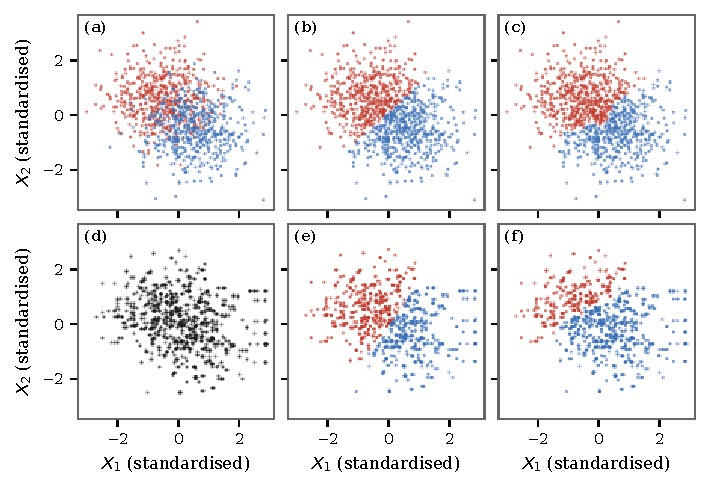
\includegraphics{figures/fig_normal.pdf}
\caption{Normal (spherical) components: geometry largely preserved under
  synthesis. Top row, original data: (a) true group labels, (b) $k$-means
  partition, (c) Ward partition. Bottom row, the corresponding CART synthetic
  dataset: (d) synthetic group label, (e) $k$-means partition, (f) Ward
  partition. The data shown are replicate 1 of the scenario $k = 2$, $p = 2$,
  $\rho = 0$, $\sigma = 2$ and its first synthetic draw; axes are the two
  standardised features. In the partition panels, colours are matched across
  rows by Hungarian alignment, so the same colour denotes corresponding groups
  in the original and synthetic panels. Panel (d) is drawn in a single colour:
  the group label in the synthetic data is itself synthesised, so it is a
  prediction from the synthetic features rather than a planted truth, and it
  has no bijective correspondence with the original groups. Both rows contain
  the same number of observations ($N = 1000$); the synthetic panels can look
  sparser only because CART resamples observed values, so that points coincide
  more often.}
\label{fig:normal}
\end{figure}

\begin{figure}[t]
\centering
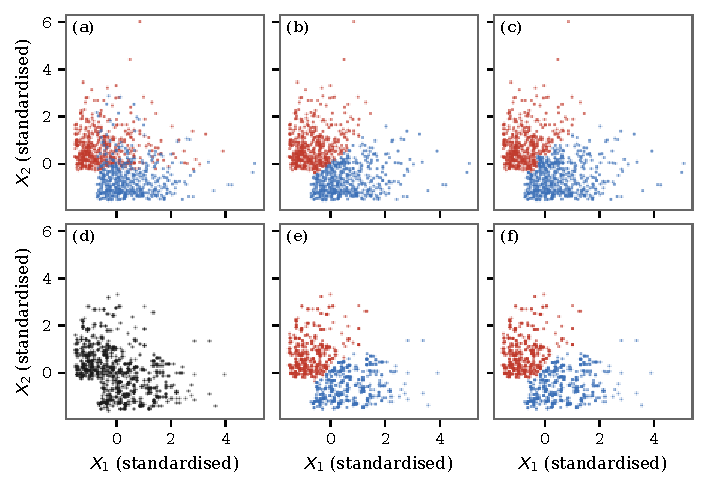
\includegraphics{figures/fig_gamma.pdf}
\caption{Gamma (right-skewed) components: the same synthesis mechanism breaks
  smooth tails into axis-aligned blocks. Panel layout (a)--(f), colour
  matching, the single-colour panel (d), the replicate and draw shown, and the
  scenario ($k = 2$, $p = 2$, $\rho = 0$, $\sigma = 2$) are as in
  Fig.~\ref{fig:normal}, and both rows again contain $N = 1000$ observations.
  Comparing panel (d) with panel (a) shows the artefact directly: the
  continuous density gradient of the original becomes a set of discrete
  rectangular patches.}
\label{fig:gamma}
\end{figure}

\subsection{Number of groups}
\label{sec:count}

The number of clusters estimated from synthetic data can be evaluated against
two references, each addressing a different question
(Section~\ref{sec:metrics}). Comparison with the planted number of groups
($\mathrm{RR}$) assesses whether the synthetic data support recovery of the
underlying truth, and so combines synthesis distortion with the inability of
the clustering procedure to find the planted structure at all. Comparison with
the number estimated from the original data ($\mathrm{AG}$) removes the second
component but retains the ordinary resampling instability of $\hat{k}$, which
the bootstrap null measures (Section~\ref{sec:excess}). Both references are
reported throughout, and Figure~\ref{fig:recovery} shows each against
separation, stratified by the true number of groups.

Separation is the decisive factor under both references. Against the planted
number of groups, recovery rises from $0.247$ ($k$-means) and $0.281$ (Ward)
at $\sigma = 0.1$, through $0.288$ and $0.295$ at $\sigma = 2$, to $0.810$ and
$0.789$ at $\sigma = 6$ and $0.954$ and $0.950$ at $\sigma = 10$. The
transition is sharp: up to $\sigma = 2$ recovery is low and dominated by the
overlap of the groups themselves, while at $\sigma = 10$ it is high for every
$k$.

Against the number estimated from the original data the picture is markedly
more favourable, and the gap is largest exactly where the groups overlap:
agreement is $0.684$ ($k$-means) and $0.646$ (Ward) at $\sigma = 0.1$, rising
to $0.982$ and $0.975$ at $\sigma = 10$, for overall agreement of $0.839$ and
$0.811$. The explanation is that at low separation the algorithms frequently
fail to recover the planted count from the original data as well: at
$\sigma = 0.1$, $k$-means finds the true $k$ in only $0.233$ of original
datasets and Ward in $0.294$. Much of what the first reference records as a
failure of synthesis is therefore a failure of clustering under overlap, which
synthesis reproduces.

The number of groups behaves very differently under the two references.
Against the planted count, recovery is much higher for fewer groups: $0.819$
for $k$-means at $k = 2$, against $0.468$ at $k = 3$ and $0.437$ at $k = 4$;
in the overlapping regime the three- and four-group cases are almost never
recovered (at most $0.12$), yet they exceed $0.90$ once $\sigma = 10$. Against
the original data, this pattern largely disappears ($0.847$, $0.838$ and
$0.833$). The difficulty of larger $k$ thus lies mainly in the clustering
problem, which synthesis reproduces, rather than in synthesis itself. The
partial $\eta^2$ values from the main-effects model make the contrast
explicit: for the planted reference, separation ($0.565$ for $k$-means,
$0.577$ for Ward) and $k$ ($0.287$ and $0.357$) dominate, whereas for
agreement with the original data separation ($0.245$ and $0.229$) is followed
by correlation ($0.141$ and $0.075$) and distribution family ($0.019$ and
$0.105$), with $k$ below $0.001$. For agreement, however, the main effects
explain only a third of the variation ($R^2 = 0.340$ and $0.349$); adding all
two-way interactions raises $R^2$ to $0.606$ and $0.605$, with large
correlation-by-separation terms ($0.282$ and $0.179$), so the ranking
describes average tendencies rather than a separable structure.
Table~\ref{tab:factors} reports the marginal means for every design factor
under both references.

\begin{figure}[t]
\centering
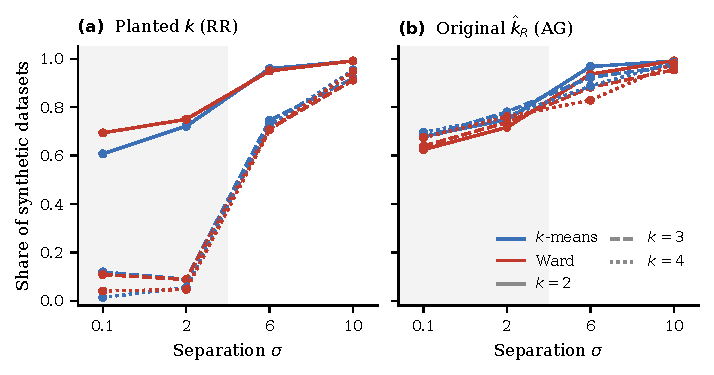
\includegraphics{figures/fig_recovery.pdf}
\caption{Cluster-count agreement between synthetic and original data, against
  separation and stratified by the true number of groups, under two reference
  conventions: (a) agreement with the number of groups planted by the
  simulation ($\mathrm{RR}$); (b) agreement with the number the same
  algorithm recovers from the original data ($\mathrm{AG}$). The separation
  levels are shown as categories because they are not equally spaced; the
  shaded region marks overlapping groups ($\sigma \le 2$). In (a), agreement is
  low while the groups overlap for $k \ge 3$ and moderate for $k = 2$; (b)
  stays higher throughout and depends far less on $k$, because in the
  overlapping regime the algorithms often fail to recover the planted count
  from the original data as well. Candidate range $\{2,\dots,8\}$; each point
  pools 60{,}000 original--synthetic pairs.}
\label{fig:recovery}
\end{figure}

\begin{table}[t]
\centering
\caption{Agreement in the number of groups by design factor, over the full
         720{,}000-evaluation design, under the two references of
         Eq.~\eqref{eq:sr}: the planted number of groups ($\mathrm{RR}$) and
         the number estimated from the original data ($\mathrm{AG}$). Each
         entry is a marginal mean over all other factors; candidate range
         $\{2,\dots,8\}$. Wilcoxon $p$: paired signed-rank test of $k$-means
         against Ward across the 144 scenario-level means. The capped range
         $\{2,\dots,\min(k+3,8)\}$ is reported in Supplementary Table~S2.}
\label{tab:factors}
\small
\begin{tabular}{llrrrr}
\toprule
 & & \multicolumn{2}{c}{Planted $k$ (RR)} & \multicolumn{2}{c}{Original $\hat{k}_R$ (AG)} \\
\cmidrule(lr){3-4}\cmidrule(lr){5-6}
Factor & Level & $k$-means & Ward & $k$-means & Ward \\
\midrule
Separation $\sigma$ & $0.1$\textsuperscript{a} & 0.247 & 0.281 & 0.684 & 0.646 \\
 & $2$\textsuperscript{a} & 0.288 & 0.295 & 0.764 & 0.738 \\
 & $6$ & 0.810 & 0.789 & 0.926 & 0.882 \\
 & $10$ & 0.954 & 0.950 & 0.982 & 0.975 \\
\addlinespace
Number of groups $k$ & $2$ & 0.819 & 0.846 & 0.847 & 0.817 \\
 & $3$ & 0.468 & 0.455 & 0.838 & 0.803 \\
 & $4$ & 0.437 & 0.435 & 0.833 & 0.811 \\
\addlinespace
Dimensionality $p$ & $2$ & 0.605 & 0.613 & 0.817 & 0.756 \\
 & $5$ & 0.554 & 0.563 & 0.849 & 0.806 \\
 & $10$ & 0.565 & 0.560 & 0.851 & 0.870 \\
\addlinespace
Correlation $\rho$ & $0$ & 0.553 & 0.567 & 0.753 & 0.744 \\
 & $0.4$ & 0.597 & 0.590 & 0.925 & 0.877 \\
\addlinespace
Distribution $F$ & Normal & 0.593 & 0.604 & 0.869 & 0.890 \\
 & Gamma & 0.557 & 0.554 & 0.809 & 0.731 \\
\midrule
Overall & & 0.575 & 0.579 & 0.839 & 0.811 \\
Wilcoxon $p$ & & \multicolumn{2}{c}{0.750} & \multicolumn{2}{c}{$5.4\times10^{-5}$} \\
\bottomrule
\end{tabular}

\par\smallskip
\begin{minipage}{0.92\linewidth}\footnotesize
\textsuperscript{a}All collapse cells lie at $\sigma \le 2$: scenarios with
$k \ge 3$ in which every original dataset gives $\hat{k}_R = 2$ (22 of 96 for
$k$-means, 26 of 96 for Ward). They contain $15.3\%$ and $18.1\%$ of all
evaluations, and agreement is $0.955$ and $0.929$ inside them against $0.799$
and $0.762$ outside (Supplementary Section~S6).
\end{minipage}
\end{table}

Three further patterns in Table~\ref{tab:factors} deserve comment. First,
agreement with the original data is higher for correlated components
($0.925$ versus $0.753$ for $k$-means; $0.877$ versus $0.744$ for Ward), but
this is an effect of the estimator rather than of synthesis. At
$\sigma \le 2$ the silhouette scan returns $\hat{k}_R = 2$ for $91.1\%$
($k$-means) and $87.8\%$ (Ward) of original datasets with $\rho = 0.4$,
against $38.3\%$ and $62.2\%$ with $\rho = 0$, so original and synthetic
estimates coincide largely because both collapse onto the smallest candidate.
Where the estimator is not collapsed ($\sigma \ge 6$), agreement is slightly
lower for correlated components ($0.948$ versus $0.960$ for $k$-means;
$0.914$ versus $0.944$ for Ward). Second, dimensionality has opposite effects
in the two regimes. At $\sigma \le 2$ Ward's agreement rises with $p$ ($0.536$,
$0.703$ and $0.839$ at $p = 2$, $5$ and $10$), again because of collapse: at
$p = 10$ and $\sigma \le 2$ the scan selects $\hat{k}_R = 2$ for $80.8\%$
($k$-means) and $90.0\%$ (Ward) of original datasets. At $\sigma = 6$, where
the groups are separated but not trivially so, agreement falls with $p$
($k$-means $0.976$, $0.903$ and $0.899$; Ward $0.976$, $0.853$ and $0.818$).
Third, the collapse cells marked in Table~\ref{tab:factors}, a sixth of the
design, contribute near-automatic agreement and raise the overall values. The
distribution family produces a consistent gap under both references, which
Section~\ref{sec:distribution} examines.

\subsection{Agreement relative to the bootstrap null}
\label{sec:excess}

Table~\ref{tab:null} sets $\mathrm{AG}$ beside its bootstrap null. Both
algorithms agree with the original estimate less often after synthesis than
after bootstrap resampling: overall $\mathrm{AG}_0$ is $0.871$ for $k$-means
and $0.826$ for Ward, so the excess is $-0.032$ and $-0.016$. Synthetic
agreement lies below the null in 99 of the 144 scenarios for $k$-means
(10 above, 35 ties; Wilcoxon $p = 1.1 \times 10^{-11}$) and in 90 for Ward
(30 above, 24 ties; $p = 4.8 \times 10^{-6}$). The loss attributable to CART
beyond resampling is therefore real but small, a few points of agreement,
against a resampling instability that is already sizeable: even a bootstrap
resample of the original fails to reproduce $\hat{k}_R$ in $12.9\%$ of cases
for $k$-means and $17.4\%$ for Ward. Two independent original datasets
from the same scenario, a coarser reference that also changes the centroid
geometry, agree in $0.801$ and $0.767$ of pairs (Supplementary Section~S4).

\begin{table}[t]
\centering
\caption{Agreement with the original estimate after CART synthesis
         ($\mathrm{AG}$) and after bootstrap resampling of the original data
         ($\mathrm{AG}_0$, $B = 30$ resamples per original dataset), and the
         excess $\mathrm{AG} - \mathrm{AG}_0$; negative values mean that
         synthesis loses agreement beyond resampling. Candidate range
         $\{2,\dots,8\}$. The excess is computed before rounding.}
\label{tab:null}
\small
\begin{tabular}{llrrrrrr}
\toprule
 & & \multicolumn{3}{c}{$k$-means} & \multicolumn{3}{c}{Ward} \\
\cmidrule(lr){3-5}\cmidrule(lr){6-8}
Stratum & Level & AG & AG$_0$ & Excess & AG & AG$_0$ & Excess \\
\midrule
Separation $\sigma$ & $0.1$ & 0.684 & 0.721 & $-0.038$ & 0.646 & 0.644 & $+0.002$ \\
 & $2$ & 0.764 & 0.814 & $-0.051$ & 0.738 & 0.754 & $-0.016$ \\
 & $6$ & 0.926 & 0.960 & $-0.034$ & 0.882 & 0.923 & $-0.040$ \\
 & $10$ & 0.982 & 0.989 & $-0.007$ & 0.975 & 0.984 & $-0.009$ \\
\addlinespace
Distribution $F$ & Normal & 0.869 & 0.880 & $-0.011$ & 0.890 & 0.902 & $-0.012$ \\
 & Gamma & 0.809 & 0.863 & $-0.053$ & 0.731 & 0.750 & $-0.020$ \\
\addlinespace
Normal, $\sigma$ & $0.1$ & 0.665 & 0.655 & $+0.011$ & 0.782 & 0.773 & $+0.009$ \\
 & $2$ & 0.879 & 0.903 & $-0.024$ & 0.873 & 0.886 & $-0.013$ \\
 & $6$ & 0.947 & 0.974 & $-0.028$ & 0.924 & 0.964 & $-0.040$ \\
 & $10$ & 0.983 & 0.988 & $-0.005$ & 0.982 & 0.986 & $-0.004$ \\
\addlinespace
Gamma, $\sigma$ & $0.1$ & 0.702 & 0.788 & $-0.086$ & 0.511 & 0.515 & $-0.004$ \\
 & $2$ & 0.648 & 0.726 & $-0.078$ & 0.603 & 0.623 & $-0.019$ \\
 & $6$ & 0.906 & 0.946 & $-0.040$ & 0.841 & 0.881 & $-0.041$ \\
 & $10$ & 0.981 & 0.991 & $-0.010$ & 0.969 & 0.983 & $-0.014$ \\
\midrule
Overall &  & 0.839 & 0.871 & $-0.032$ & 0.811 & 0.826 & $-0.016$ \\
\bottomrule
\end{tabular}

\end{table}

\subsection{Geometric fidelity}
\label{sec:geometry}

Figure~\ref{fig:fidelity} traces the geometric-fidelity metrics against
separation, together with their bootstrap floors, and
Table~\ref{tab:floor} summarises them. Mean centroid distance falls steeply as
groups separate, from $0.604$ ($k$-means) and $0.859$ (Ward) at
$\sigma = 0.1$ to $0.090$ and $0.095$ at $\sigma = 10$, and mean variance
difference falls from $0.353$ and $0.613$ to $0.112$ and $0.133$. Observed
values are lower for $k$-means in 133 of the 144 scenarios for MCD, in all 144
for MVD and in 138 for $\Delta G$ (paired Wilcoxon $p < 10^{-20}$ for each).

Most of this distortion, however, is already produced by resampling.
Bootstrap resampling alone reproduces $0.222$ of the $0.303$ observed MCD for
$k$-means and $0.403$ of $0.460$ for Ward, $0.150$ of $0.219$ and $0.324$ of
$0.392$ for MVD, and $0.021$ of $0.030$ and $0.053$ of $0.061$ for $\Delta G$,
and the floor already places $k$-means below Ward (in 121, 135 and 132 of the
144 scenarios for MCD, MVD and $\Delta G$). CART adds a positive excess in
almost every scenario (MCD 144 and 143 of 144 for $k$-means and Ward; MVD 144
and 141; $\Delta G$ 144 and 129; $p < 10^{-20}$ for each), but the excess is
not smaller for $k$-means: it is larger for MCD ($0.081$ versus $0.057$;
Wilcoxon $p = 8.8 \times 10^{-6}$) and equal for MVD ($0.069$ versus $0.068$;
$p = 0.973$) and for $\Delta G$ ($0.009$ versus $0.008$; $p = 0.462$). The
lower geometric distortion of $k$-means on synthetic data is therefore
inherited from its lower distortion under resampling, not produced by a
smaller effect of CART.

The scale-free metrics correct the reading of the separation trend. In units
of the within-component standard deviation, the centroid displacement still
falls with separation ($k$-means $0.605$ to $0.189$; Ward $0.860$ to $0.201$),
and CART moves the centroids by about $0.10$ ($k$-means) and $0.08$ (Ward)
within-component standard deviations beyond resampling. Dispersion behaves
differently. The relative variance difference shows that a synthetic
cluster's dispersion deviates from the original's by $8.2\%$ on average for
$k$-means and $15.2\%$ for Ward, of which $5.5$ and $12.6$ points are
resampling; the excess attributable to CART is about $2.7$ points for both
($0.027$ versus $0.026$; $p = 0.891$). This excess does not decline with
separation; it grows ($k$-means $0.022$, $0.021$, $0.030$ and $0.035$ across
the four levels of $\sigma$; Ward $0.015$, $0.013$, $0.036$ and $0.041$). The
decline of absolute MVD with $\sigma$ is thus mostly a decline of the floor
and a change of units, not a reduction of the dispersion distortion that CART
introduces.

\begin{figure}[t]
\centering
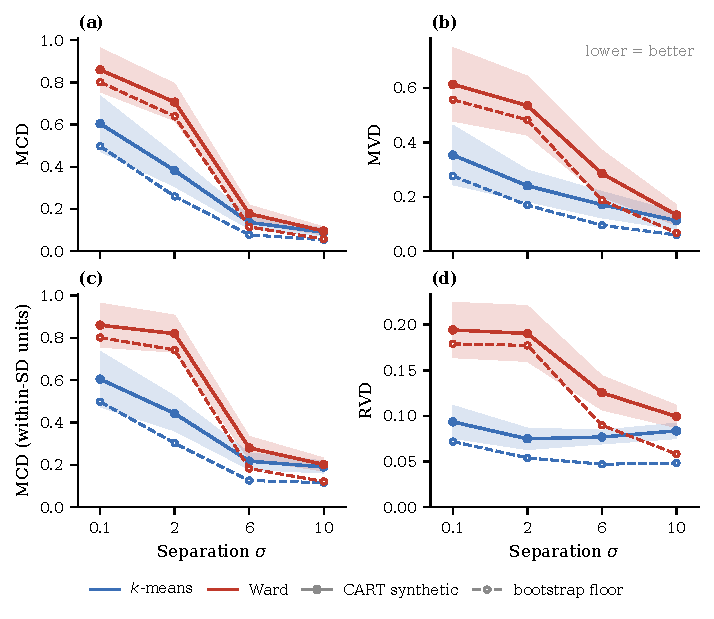
\includegraphics{figures/fig_fidelity.pdf}
\caption{Geometric fidelity against separation, observed after CART synthesis
  (solid lines, filled markers) and under bootstrap resampling of the original
  data (dashed lines, open markers; $B = 30$). (a) Mean centroid distance and
  (b) mean variance difference, in the units of the scaler fit on the
  original data; (c) mean centroid distance in units of the within-component
  standard deviation ($\mathrm{MCD}_{\mathrm{sd}}$); (d) relative variance
  difference (RVD). Points are means of the 36 scenario-level means at each
  separation level; bands are $\pm 1.96$ standard errors across those
  scenarios and describe the spread over the design, not sampling
  uncertainty. The vertical distance between a solid and a dashed line of the
  same colour is the excess attributable to CART.}
\label{fig:fidelity}
\end{figure}

\begin{table}[t]
\centering
\caption{Geometric fidelity after CART synthesis (observed), under bootstrap
         resampling of the original data (floor, $B = 30$) and their
         difference (excess), averaged over the 144 scenario means, at the
         planted $k$. MCD, MVD and $\Delta G$ are in the units of the scaler
         fit on the original data; $\mathrm{MCD}_{\mathrm{sd}}$ is in
         within-component standard deviations and RVD is a relative error.
         Last column: Wilcoxon $p$ for the excess of $k$-means against the
         excess of Ward across the 144 scenarios. Values by separation,
         distribution family and dimensionality are in Supplementary
         Section~S5.}
\label{tab:floor}
\small
\begin{tabular}{lrrrrrrr}
\toprule
 & \multicolumn{3}{c}{$k$-means} & \multicolumn{3}{c}{Ward} & Excess \\
\cmidrule(lr){2-4}\cmidrule(lr){5-7}
Metric & Observed & Floor & Excess & Observed & Floor & Excess & $p$ \\
\midrule
MCD & 0.303 & 0.222 & 0.081 & 0.460 & 0.403 & 0.057 & $8.8\times10^{-6}$ \\
MVD & 0.219 & 0.150 & 0.069 & 0.392 & 0.324 & 0.068 & 0.973 \\
$\Delta G$ & 0.030 & 0.021 & 0.009 & 0.061 & 0.053 & 0.008 & 0.462 \\
\addlinespace
MCD$_{\mathrm{sd}}$ & 0.363 & 0.260 & 0.103 & 0.540 & 0.462 & 0.078 & $2.7\times10^{-5}$ \\
RVD & 0.082 & 0.055 & 0.027 & 0.152 & 0.126 & 0.026 & 0.891 \\
\bottomrule
\end{tabular}

\end{table}

Total dispersion distortion grows with dimensionality.
Figure~\ref{fig:balance}(a) shows MVD rising with the number of variables: for
$k$-means from $0.06$ ($95\%$ interval $0.05$--$0.08$) at $p = 2$ to $0.39$
($0.32$--$0.47$) at $p = 10$, and for Ward from $0.13$ to $0.65$. Because $v_j$
in Eq.~\eqref{eq:mvd} is a sum of squared deviations over the $p$ coordinates,
this growth should be read per coordinate: $\mathrm{MVD}/p$ is roughly constant
($k$-means $0.032$, $0.040$ and $0.039$ at $p = 2, 5, 10$; Ward $0.067$,
$0.078$ and $0.065$). The floor grows in the same way ($k$-means $0.047$,
$0.144$ and $0.259$), so much of the accumulation is resampling noise summed
over coordinates; the per-coordinate excess attributable to CART increases
only mildly with $p$ ($k$-means $0.008$, $0.011$ and $0.013$; Ward $0.006$,
$0.010$ and $0.014$). Unlike the count, which is protected at high $p$ and low
$\sigma$ by the collapse of $\hat{k}$ onto small values
(Section~\ref{sec:count}), the within-cluster dispersion is measured at the
planted $k$ and so exposes this accumulation directly.

Figure~\ref{fig:balance}(b) shows the group-balance error $\Delta G$ by
distribution family. Both algorithms preserve cluster sizes better on Normal
than on Gamma data ($k$-means $0.028$ versus $0.032$; Ward $0.057$ versus
$0.065$), consistent with the block artefact being more disruptive on skewed
groups. $k$-means yields systematically lower $\Delta G$ than Ward for both
distributions (lower in 138 of 144 scenarios; overall $0.030$ versus $0.061$),
but the floor shows the same ordering ($0.021$ versus $0.053$): because the
planted groups have equal sizes, the difference reflects the fact that the
cluster sizes of a $k$-means partition fluctuate less under resampling, and
hence also under synthesis. This is consistent with the known tendency of the
$k$-means criterion to produce clusters of similar size \citep{xiong2009}.
Whether $k$-means would also understate a genuine size imbalance cannot be
tested with balanced groups, and is left to future work
(Section~\ref{sec:future}).

\begin{figure}[t]
\centering
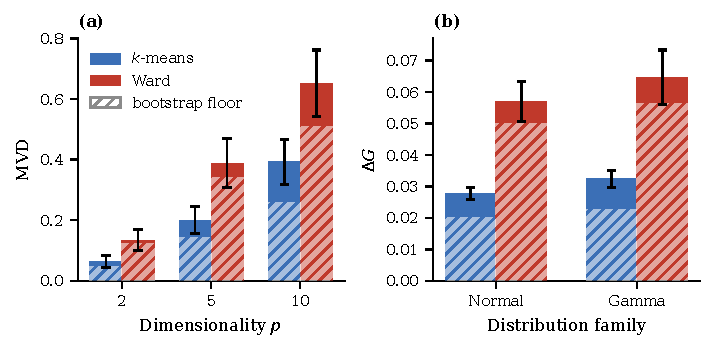
\includegraphics{figures/fig_balance.pdf}
\caption{(a) Mean variance difference by dimensionality: total distortion
  accumulates as dimensions are added, more so for Ward; per coordinate it is
  roughly constant (see text). (b) Group-balance error $\Delta G$ by
  distribution family. Solid bars are the observed means of the scenario-level
  means after CART synthesis; the hatched inner bars are the bootstrap floor
  ($B = 30$), so the solid part above each hatched bar is the excess
  attributable to CART. Error bars are $\pm 1.96$ standard errors of the
  observed values across scenarios (48 per level of $p$, 72 per
  distribution).}
\label{fig:balance}
\end{figure}

\subsection{Distribution family}
\label{sec:distribution}

The distribution family is the factor that exposes the CART artefact most
directly. Figure~\ref{fig:distribution} stratifies count agreement by
distribution and separation under both references, each shown with its
reference on data without synthesis. Against the planted number of groups
(panels a and b), the two families show similar recovery while the groups
overlap and diverge at intermediate separation: at $\sigma = 6$, $k$-means
recovers the planted count $86.2\%$ of the time for Normal data but only
$75.9\%$ for Gamma data (Ward: $84.5\%$ versus $73.2\%$). Almost all of this
gap, however, is already present in the original data, where the planted
count is recovered in $90.0\%$ versus $80.0\%$ of datasets ($k$-means; Ward
$91.1\%$ versus $78.9\%$). It therefore reflects mainly how difficult skewed
groups are to cluster, not what synthesis does to them.

Against the original data (panels c and d), the Gamma penalty is concentrated
where the groups overlap and is much larger for Ward. At $\sigma = 0.1$,
Ward's agreement is $0.782$ for Normal but only $0.511$ for Gamma data, and at
$\sigma = 2$ it is $0.873$ versus $0.603$; the corresponding values for
$k$-means are $0.665$ versus $0.702$ and $0.879$ versus $0.648$. At
$\sigma = 6$ the gap narrows ($k$-means $0.947$ versus $0.906$; Ward $0.924$
versus $0.841$), and at $\sigma = 10$ a small gap remains for Ward ($0.982$
versus $0.969$; $k$-means $0.983$ versus $0.981$). The bootstrap null shows
where this penalty comes from. For Ward, the null already contains it:
$\mathrm{AG}_0$ is $0.515$ for Gamma and $0.773$ for Normal data at
$\sigma = 0.1$, so the low agreement of Ward on skewed, overlapping data is an
instability of its silhouette estimate that synthesis inherits, and the
Gamma excess is small at every separation (between $-0.041$ and $-0.004$). For
$k$-means the null is higher on Gamma data ($0.788$ at $\sigma = 0.1$ and
$0.726$ at $\sigma = 2$), and the loss attributable to CART is largest exactly
there ($-0.086$ and $-0.078$).

This addresses the first objective. CART preserves the structure needed to
recover the number of groups on Normal data to within about one point of the
bootstrap null (excess $-0.011$ for $k$-means and $-0.012$ for Ward), and its
hardening of skewed densities lowers agreement on Gamma data beyond
resampling, most markedly for $k$-means when groups overlap. The larger Gamma
penalty seen for Ward in the raw agreement is mainly the instability of its
estimate on skewed, overlapping data rather than a larger effect of CART.

\begin{figure}[t]
\centering
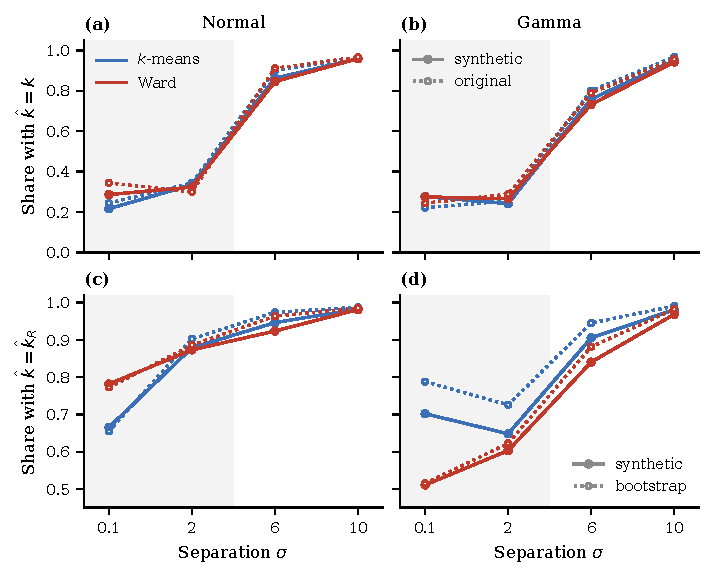
\includegraphics{figures/fig_distribution.pdf}
\caption{Cluster-count agreement by distribution family (columns: Normal,
  Gamma) and separation, under the two references (candidate range
  $\{2,\dots,8\}$). (a, b) Share of synthetic datasets with
  $\hat{k}_S = k$ (RR; solid) beside the share of original datasets with
  $\hat{k}_R = k$ (dotted, open markers). (c, d) Share of synthetic datasets
  with $\hat{k}_S = \hat{k}_R$ (AG; solid) beside the share of bootstrap
  resamples with $\hat{k}_b = \hat{k}_R$ ($\mathrm{AG}_0$; dotted, open
  markers). The vertical distance between a solid and a dotted line of the
  same colour is the part of the disagreement attributable to CART. Separation
  is shown as a categorical axis; the shaded region marks $\sigma \le 2$.}
\label{fig:distribution}
\end{figure}

\subsection{Agreement between the two algorithms}
\label{sec:algo}

Whether the two methods differ in robustness to synthetic distortion was the
third objective, and the answer depends on the reference. Against the planted
number of groups the two are indistinguishable: overall recovery is $0.575$
for $k$-means and $0.579$ for Ward, a paired Wilcoxon signed-rank test across
the 144 scenario-level means finds no significant difference ($W = 3508.5$,
$p = 0.750$), and the two algorithms reach the same outcome in $92.0\%$ of
individual evaluations.

Against the original data, $k$-means reproduces the number of groups more
often than Ward: overall agreement is $0.839$ versus $0.811$, $k$-means is
higher in 90 of the 144 scenarios (30 lower, 24 ties), and the paired test is
significant ($W = 2088.5$, $p = 5.4 \times 10^{-5}$). For an analyst who will
cluster a synthetic release, this is the practically relevant comparison, and
it is not uniform. The advantage of $k$-means arises on Gamma data ($0.809$
versus $0.731$; higher in 59 of 72 scenarios, $p = 2.6 \times 10^{-6}$),
where it is significant at $\sigma = 0.1$ ($0.702$ versus $0.511$,
$p = 0.002$), $\sigma = 6$ ($0.906$ versus $0.841$, $p = 0.001$) and
$\sigma = 10$ ($0.981$ versus $0.969$, $p = 0.006$) but not at $\sigma = 2$
($0.648$ versus $0.603$, $p = 0.099$). On Normal data there is no difference
($0.869$ versus $0.890$, $p = 0.595$), and in the most overlapping Normal
scenarios Ward is numerically higher ($0.782$ versus $0.665$ at
$\sigma = 0.1$; $p = 0.136$). The conclusion is unchanged under the capped
candidate range (Supplementary Section~S3).

The bootstrap null shows why. The same advantage is already present without
synthesis: $\mathrm{AG}_0$ is $0.871$ for $k$-means against $0.826$ for Ward
($W = 966$, $p = 6.0 \times 10^{-5}$), and $0.863$ against $0.750$ on Gamma
data ($p = 6.3 \times 10^{-7}$), while on Normal data the nulls do not differ
($0.880$ versus $0.902$, $p = 0.900$). The silhouette-based estimate of $k$ is
more stable under resampling for $k$-means, particularly on skewed data, and
synthesis inherits that stability. Beyond resampling, $k$-means loses slightly
more agreement than Ward (difference in excess $-0.017$, $W = 2846$,
$p = 0.040$), again only on Gamma data ($-0.034$, $p = 0.024$; concentrated at
$\sigma = 0.1$, $-0.082$, and $\sigma = 2$, $-0.058$), with no difference on
Normal data ($p = 0.640$); with 30 resamples per dataset these excess
comparisons are modest evidence. The higher agreement of $k$-means on
synthetic data thus reflects the greater stability of its $\hat{k}$, not
smaller damage from CART, and the same holds for the geometric metrics
(Section~\ref{sec:geometry}).

As a complementary check on internal cohesion, the difference in mean
silhouette width between synthetic and original partitions at the planted $k$
is small and centred near zero at every separation (at most $0.0125$ in
absolute value, for Ward at $\sigma = 0.1$). The absolute levels are nearly
identical ($k$-means $0.396$ versus $0.397$; Ward $0.376$ versus $0.377$),
suggesting that the apparent clustering quality is similar before and after
synthesis. This is reassuring, but it also means that silhouette alone would
fail to flag the geometric distortions the other metrics detect, an
instructive negative result for anyone tempted to validate a synthetic release
with an internal index.

% =====================================================================
\section{Discussion}
% =====================================================================

This study evaluated whether CART-generated synthetic data preserve the
structural properties that cluster analysis relies on, comparing $k$-means and
Ward's hierarchical clustering across a 144-scenario factorial design and
720{,}000 synthetic-versus-original evaluations, each read against a bootstrap
resample of the same original data. Four findings emerge.

First, separation dominates agreement in the number of groups. Agreement with
the original data rises from $0.684$ ($k$-means) and $0.646$ (Ward) when the
groups overlap to $0.982$ and $0.975$ when they are well separated, and
recovery of the planted count rises from $0.247$ and $0.281$ to $0.954$ and
$0.950$. The number
of groups strongly affects recovery of the planted count ($0.819$ at $k = 2$
against $0.468$ and $0.437$ at $k = 3$ and $4$, for $k$-means) but has little
effect on agreement between original and synthetic estimates. Most of the
effect of $k$ is a property of the clustering problem that synthesis
reproduces rather than a distortion that synthesis introduces. Where groups
overlap, a sixth of the design consists of collapse cells in which the
silhouette scan returns two groups for every original dataset, and agreement
there is close to automatic.

Second, for a researcher who clusters a synthetic release, $k$-means
reproduces the number of groups found in the original data more often than
Ward's linkage ($0.839$ versus $0.811$). This happens on skewed Gamma data
($0.809$ versus $0.731$), at every separation except $\sigma = 2$, and not on
Normal data ($0.869$ versus $0.890$). The bootstrap null shows that this
advantage reflects the greater stability of the $k$-means estimate of $k$
under resampling ($\mathrm{AG}_0$ $0.871$ versus $0.826$), not smaller damage
from CART: the agreement lost to synthesis beyond resampling is small for
both methods ($0.032$ and $0.016$) and, if anything, slightly larger for
$k$-means. The geometry tells the same story. $k$-means shows lower centroid,
dispersion and cluster-size distortion on synthetic data, but most of each
metric is reproduced by resampling alone, and the excess attributable to CART
is not smaller for $k$-means (larger for MCD, equal for MVD, $\Delta G$ and
RVD). For an applied analyst, the practical implication is that the choice of
algorithm matters more for the fidelity of a synthetic-data analysis than
accuracy against a ground truth would suggest, and that the reason is the
stability of the estimator rather than the generator.

Third, CART is not utility-neutral, and its effect depends on the underlying
distribution. On Normal data the count agreement after synthesis is within
about one point of the bootstrap null; on skewed Gamma data CART hardens smooth
density gradients into axis-aligned blocks, visibly distorting geometry and
lowering agreement beyond resampling, most for $k$-means when groups overlap.
CART adds a positive excess over the resampling floor to every geometric
metric in almost every scenario; in relative terms it changes within-cluster
dispersion by about $2.7\%$ beyond resampling, and this relative excess grows
rather than shrinks with separation.

Fourth, and methodologically, neither an internal validity index nor raw
agreement is a sufficient check. Silhouette values remain almost unchanged
even where centroid and dispersion fidelity degrade. A practitioner who
validates a synthetic release by confirming that its silhouette profile
matches the original may conclude that structure is intact in precisely the
settings where this analysis shows it is not. Raw agreement, in turn, mixes
the effect of the generator with the instability of the estimator, and the
comparison between algorithms changes once each method is set against its own
resampling null. The planted truth, the natural choice in a simulation,
answers yet another question, and in this study it masked the difference
between the two algorithms.

An interesting corollary of the design is that clustering can be read in the
other direction, as an instrument rather than an object of study. Because a
partition responds to local density, separability and dispersion
simultaneously, the agreement between partitions recovered from original and
synthetic data functions as a sensitive summary of geometric resemblance, one
that reacts to distortions which marginal and bivariate checks may not detect.
We did not pursue this here, but the metrics of Section~\ref{sec:metrics} could
be repurposed as general-utility diagnostics rather than task-specific ones.

\subsection{Relation to previous work}

The study extends \citet{chen2025} in three ways: a second algorithm that
shares the criterion of $k$-means but optimises it differently, a skewed
distribution family that exposes tree-synthesis artefacts, and structural
metrics that compare partitions recovered from the original and synthetic
data. It should be distinguished from the cluster-based utility measure of
\citet{woo2009}, which clusters the merged original and masked records and
measures how well each cluster mixes the two sources; that measure uses
clustering as a device for general utility, whereas we ask whether a
clustering analysis of the release reproduces the analysis of the original.
The conclusion that CART is a reasonable default for well-behaved data but
degrades on skewed distributions is consistent with the broader
\texttt{synthpop} literature \citep{nowok2016,snoke2018}, and the qualitative
block artefact matches the known axis-aligned bias of sequential tree
synthesis. The finding that utility rankings depend on the downstream task
echoes benchmarking work in the health-records setting
\citep{yan2022,elemam2022}, where the same generator changes position depending
on which analysis is used to score it, and an applied study of wearable
physiological data in mental-health monitoring similarly found that the
clustering utility of \texttt{synthpop} releases depends on the synthesis
settings \citep{vidiella2025}. The lower stability of Ward's estimate under
resampling is consistent with, although not directly comparable to, the
classical perturbation experiments of \citet{milligan1980}, which found that
methods differ in their sensitivity to error perturbation. A parallel question
arises when values are missing rather than synthesised: \citet{aschenbruck2023}
evaluate how imputation strategies affect the clusters subsequently recovered
from mixed-type data, and reach a structurally similar conclusion, that the
imputation model and the clustering method interact and cannot be assessed in
isolation. Since CART underlies both sequential synthesis and widely used
non-parametric imputation, the two literatures are closer than their
vocabularies suggest.

The count-agreement measure AG is, in effect, a stability criterion. A long
line of work validates clusterings, and chooses their number, by asking how
reproducibly a partition is recovered when the data are perturbed: by
subsampling \citep{levine2001,benhur2002}, by prediction from one half of the
sample to the other \citep{dudoit2002,lange2004,tibshirani2005,wang2010}, or by
the bootstrap \citep{jain1987,hennig2007,fang2012}; \citet{luxburg2010} reviews
these ideas. A synthetic release is a perturbation of the same kind, except
that the synthesiser, not the analyst, produces it, so AG measures the
stability of $\hat{k}$ under synthesis. Two results from this literature
govern how AG should be read. First, stability is not correctness:
\citet{bendavid2006} show that stability is driven by the structure of the
clustering objective rather than by the true number of groups, so AG must be
read together with recovery of the planted $k$; the collapse cells of
Section~\ref{sec:count}, where agreement is high because the estimator
returns two groups regardless, are an instance. Second, agreement under
perturbation has no natural zero, because $\hat{k}$ is already variable on the
original data. We therefore calibrate AG against a bootstrap null, in the
spirit of resampling-based assessments of cluster structure
\citep{suzuki2006,maitra2012}: agreement that a bootstrap resample of the
original already fails to reach cannot be attributed to CART. In this study
the calibration changes the comparison between algorithms, because the
advantage of $k$-means in AG is matched by its advantage in $\mathrm{AG}_0$. On
the analysis side, the closest analogue is validation of a clustering on
independent data \citep{ullmann2022}; a synthetic dataset can be regarded as a
validation sample that the data holder is able to release.

\subsection{Limitations}
\label{sec:limitations}

The evaluation uses controlled simulations with known ground truth rather than
real data, and its conclusions are scoped to the grid studied: correlations up
to $\rho = 0.4$, a single Gamma shape, $N = 1000$ and exactly equal group
sizes. This isolates mechanisms cleanly but limits direct generalisation to
data with missingness, mixed types, unequal group sizes and unknown
data-generating processes. The generator is limited to CART with a single
parameterisation (minimum leaf size ten, fixed variable order) and the
algorithms to $k$-means and Ward. Sample size was fixed at $N = 1000$, so
small-sample behaviour is unexamined. The number of groups is selected by the
silhouette criterion over $\hat{k} \ge 2$, so a single-cluster solution can
never be chosen, even when the groups overlap so strongly that one cluster is
the most reasonable description; other selection rules \citep{milligan1985}
may respond differently to synthesis. Count agreement is inflated where the
estimator collapses onto the smallest candidate, as happens at low $\sigma$,
high $p$ and $\rho = 0.4$, and should be read together with the bootstrap null
and the geometric metrics. The bootstrap null rests on $B = 30$ resamples per
original dataset, so comparisons of small excesses between the algorithms
carry Monte Carlo error. Every $k$-means fit uses the same seed, so the
original and synthetic fits share their initialisations. The Wilcoxon tests
and the $\pm 1.96$ standard-error bands are computed across the 144 scenarios
of a designed grid, so they compare methods over that grid rather than over a
population of scenarios.

Two conventions in the definition of MCD and MVD deserve emphasis, because both
affect the numbers themselves and not only their interpretation. The first is
what the metrics compare. Here they compare the partition recovered from the
original data against the partition recovered from the synthetic data, which is
the quantity a claim about synthesis requires; the superficially similar
practice of comparing a recovered partition against the planted labels of the
same dataset measures clustering accuracy instead, and carries no information
about the generator. The second is scale. Both metrics are computed after
standardising with a scaler fit on the pooled original data and applied
unchanged to the synthetic data, so both are expressed in units of the pooled
original feature scale. Standardising each dataset separately would rescale
away part of the distortion the metrics are meant to capture, but the common
scaler has its own dependence on the design: the pooled spread grows with
$\sigma$, so a standardised unit is a larger within-component distance at
large separation, and absolute MCD and MVD decline with $\sigma$ partly for
that reason. Neither convention is free of $\sigma$; only relative or
within-component versions are. We therefore report RVD and
$\mathrm{MCD}_{\mathrm{sd}}$ beside the absolute metrics, and read trends
across separation from them. Absolute values of MCD and MVD are not
comparable across studies that differ in either convention, and any
replication should state both explicitly. Both metrics are also unnormalised
sums over coordinates, so their absolute values grow with $p$ even at constant
per-coordinate distortion; comparisons across dimensionality should use
per-coordinate or relative versions.

\subsection{Future work}
\label{sec:future}

The central lesson generalises beyond the specific methods studied: synthetic
data utility is task-relative, and a generator that preserves marginal
resemblance need not preserve the higher-order geometry a clustering workflow
depends on. Practically, the results argue for validating structural fidelity
(distances, dispersion, separability, balance) against the intended analysis
and against a resampling reference, and for treating a clustering comparison
as a more demanding resemblance check than marginal summaries can provide.
Natural extensions include other synthesisers, such as conditional inference
trees \citep{hothorn2006}, CART with larger minimum leaf sizes, parametric
synthesisers, copulas and deep generative models; other clustering families,
in particular Gaussian mixture models with the number of components chosen by
BIC \citep{fraley2002,scrucca2016}, which can also return a single cluster, and
non-convex and density-based methods; unequal group sizes and stronger
correlations between features; varying $N$ to probe small-sample behaviour;
and chance-corrected partition comparisons such as the adjusted Rand index
\citep{hubert1985} computed on a common set of points. A promising direction
is to model the discrepancy $\Delta$ of Eq.~\eqref{eq:discrepancy} directly as
a learned function of the design factors, turning the utility surface itself
into a predictive tool.

As a concrete next step, we propose applying the same comparison to the
wearable dataset described in \citet{vidiella2025}, to which we have direct
access. Beyond providing a real-data test of the present design, this dataset
would allow a comparison that neither study can perform alone. The present work
evaluates synthesis as substitution, in which the synthetic dataset replaces
the original. The applied study instead evaluates augmentation, in which the
synthetic records are appended to the real ones and the union is clustered.
These are different operations, and their effects are currently confounded
with sample size: doubling the number of observations alters neighbourhood
parameters and silhouette values independently of any distortion introduced by
the generator. A three-way comparison of the partitions recovered from the real
data, from the synthetic data alone, and from the augmented set, evaluated with
the same metrics used here, would separate the effect of the generator from
the effect of the additional sample. It would also make it possible to test
whether the parameterisation of the generator, rather than the generator
itself, accounts for the block artefact documented in this paper, since the
applied study reports a substantial improvement in utility after replacing
CART with conditional inference trees \citep{hothorn2006} and increasing the
minimum leaf size. We regard this comparison as a natural continuation of the
present study and as a practical way of establishing which of its conclusions
generalise beyond the simulated setting.

% =====================================================================
\section{Conclusions}
% =====================================================================

% VL-EDIT (sentence 1 rewritten: the contribution is presented as empirical,
% as proposed in item MO3; the claim that the framework "does not depend on
% the simulation" is replaced by a narrower statement)
The contribution of this study is empirical, but the comparison it uses is not
tied to the simulation that illustrates it.
The quantity $\Delta(\theta_R, \theta_S)$ is defined for any reference dataset
and any generator, and the five factors varied here all have empirical
counterparts: separation corresponds to how distinct the underlying groups
are, the number of groups to the number of latent subpopulations,
dimensionality to the number of recorded variables, correlation to the
dependence between features, and the distribution family to the shape of the
observed densities.
% VL-EDIT (replaces "in an applied dataset they can be measured": k and sigma
% are properties of an unknown partition and cannot be measured directly)
In an applied dataset, dimensionality, feature correlations and marginal
skewness can be computed directly, whereas the number of groups and their
separation are properties of an unknown partition and can at best be
estimated.
% VL-EDIT (replaces "the framework can be transferred to real data without
% modification")
Transferring the comparison to real data therefore requires two adaptations:
the planted partition must be replaced by a reference obtained from the
original data, and agreement must be calibrated against a resampling null, as
done here.
We believe such a transfer would be informative rather than merely
confirmatory.
% VL-EDIT (the uncited empirical claims "routinely show correlations above
% 0.95" and "skewness values considerably higher" are reworded as
% possibilities)
Real datasets may occupy regions of the design space that the present grid
does not reach, for example correlations between related features well above
the maximum of $\rho = 0.4$ examined here, or stronger skewness than the Gamma
family produces.
They also exhibit properties the simulation excludes altogether, such
as strongly unbalanced group sizes, ambiguous missingness in which a zero may
indicate either genuine inactivity or a non-worn device, and heterogeneity
between individuals. Each of these is a plausible source of additional
distortion under sequential tree synthesis, and each would help to refine the
conclusions reported here. We consider the unbalanced case particularly
relevant, because the group-balance error $\Delta G$ and the hypothesis that
the $k$-means criterion understates imbalance can only be fully tested when a
substantial imbalance is present in the reference data.

Within the region of the design space studied here, synthetic data generated
with CART can reproduce the appearance of clustering structure while subtly
reshaping its geometry. Both algorithms recover well-separated structure
reliably and struggle together when groups overlap. Where they diverge is in
how often each reproduces, on synthetic data, the number of groups it would
have found on the original data: $k$-means does so more often, on skewed data
and not on Normal data, because its estimate is more stable under any
resampling, not because CART damages it less. The utility of synthetic data for
clustering is therefore best understood not as a property of the data but as a
property of the data--generator--algorithm triple, to be verified against a
resampling reference rather than assumed.

\backmatter

\bmhead{Supplementary information}
The online supplementary material contains the recovery heatmap by number of
groups and separation, the contingency table of original versus synthetic
estimates, the sensitivity analysis for the candidate range of $\hat{k}$, the
bootstrap null and the independent-pairs baseline by stratum, the geometric
floor and scale-free metrics by stratum, the collapse cells, the clustering
objectives, and the computational cost of the study.

\section*{Declarations}

\noindent \textbf{Funding:} [To be completed by the authors.]

\noindent \textbf{Competing interests:} [To be completed by the authors.]

\noindent \textbf{Data availability:} All data analysed in this study are
  simulated; they can be regenerated exactly from the configuration file and
  seeds distributed with the code.

\noindent \textbf{Code availability:} The full pipeline, from data generation
  through to the figures and tables reported here, is available at
  \url{https://github.com/Sterrysx/synthetic-clustering}. Every stage is driven
  from a single configuration file and can be re-executed end to end.

\noindent \textbf{Author contributions:} [To be completed by the authors.]

\bibliography{refs}

\end{document}
'
%  Without switches (`./build.sh main') this file gives the named version in
%  the normal sn-jnl layout. The JoC reference style (joc_prep/sn-joc.bst,
%  via joc_prep/joc_bib.tex) is used in every variant.
% =====================================================================
\ifdefined\SetReferee
  \documentclass[pdflatex,referee]{sn-jnl}
  % =====================================================================
%  joc_referee.tex -- Journal of Classification referee layout for sn-jnl.cls
%
%  JoC: "Submit a fully double-spaced, single-column manuscript in English,
%  using a font size of at least 12, with wide margins ..."
%
%  Usage (immediately after \documentclass):
%      \documentclass[pdflatex,referee]{sn-jnl}
%      \input{joc_referee}
%
%  Why a patch is needed: sn-jnl.cls loads article.cls without a size option
%  and then hard-codes a 10bp/12bp \normalsize (plus fixed \fontsize values
%  for the title, abstract, headings, captions and tables), so the `12pt'
%  class option has no effect; `referee' only loads setspace and calls
%  \doublespacing on that 10-pt body.  This file
%    1. re-declares the size commands with the size12.clo values (12/14.5 pt);
%    2. re-declares the class's fixed-size font hooks so the abstract,
%       keywords, headings, captions and table bodies are >= 12 pt;
%    3. sets double spacing for 12 pt (\setstretch{1.655}: 14.5 pt x 1.655
%       = 24 pt baseline = 2 x 12 pt) and double-spaced captions;
%    4. resets the page to A4, single column, 30 mm margins on all sides
%       (text block 150 mm x 237 mm), no binding offset.
%  Works with or without the `referee' option (setspace is loaded here too).
%  Table bodies are 12 pt but single-spaced inside the tabular (setspace
%  default for floats); set \jocdoublefloatstrue below to double-space them.
% =====================================================================
\makeatletter
\RequirePackage{setspace}
\newif\ifjocdoublefloats \jocdoublefloatsfalse
%
% ---- 1. size commands (values from article's size12.clo) -------------
\renewcommand\normalsize{%
   \@setfontsize\normalsize\@xiipt{14.5}%
   \abovedisplayskip 12\p@ \@plus3\p@ \@minus7\p@
   \abovedisplayshortskip \z@ \@plus3\p@
   \belowdisplayshortskip 6.5\p@ \@plus3.5\p@ \@minus3\p@
   \belowdisplayskip \abovedisplayskip
   \let\@listi\@listI}
\renewcommand\small{%
   \@setfontsize\small\@xipt{13.6}%
   \abovedisplayskip 11\p@ \@plus3\p@ \@minus6\p@
   \abovedisplayshortskip \z@ \@plus3\p@
   \belowdisplayshortskip 6.5\p@ \@plus3.5\p@ \@minus3\p@
   \def\@listi{\leftmargin\leftmargini
               \topsep 9\p@ \@plus3\p@ \@minus5\p@
               \parsep 4.5\p@ \@plus2\p@ \@minus\p@
               \itemsep \parsep}%
   \belowdisplayskip \abovedisplayskip}
\renewcommand\footnotesize{%
   \@setfontsize\footnotesize\@xpt\@xiipt
   \abovedisplayskip 10\p@ \@plus2\p@ \@minus5\p@
   \abovedisplayshortskip \z@ \@plus3\p@
   \belowdisplayshortskip 6\p@ \@plus3\p@ \@minus3\p@
   \def\@listi{\leftmargin\leftmargini
               \topsep 6\p@ \@plus2\p@ \@minus2\p@
               \parsep 3\p@ \@plus2\p@ \@minus\p@
               \itemsep \parsep}%
   \belowdisplayskip \abovedisplayskip}
\renewcommand\scriptsize{\@setfontsize\scriptsize\@viiipt{9.5}}
\renewcommand\tiny{\@setfontsize\tiny\@vipt\@viipt}
\renewcommand\large{\@setfontsize\large\@xivpt{18}}
\renewcommand\Large{\@setfontsize\Large\@xviipt{22}}
\renewcommand\LARGE{\@setfontsize\LARGE\@xxpt{25}}
\renewcommand\huge{\@setfontsize\huge\@xxvpt{30}}
\renewcommand\Huge{\@setfontsize\Huge\@xxvpt{30}}
\DeclareMathSizes{12}{12}{8}{6}
\DeclareMathSizes{\@xiipt}{\@xiipt}{8}{6}
\normalsize
%
% ---- 2. fixed-size hooks of sn-jnl.cls -------------------------------
% (all body-type material at 12 pt; title/section heads scaled up)
\def\Artcatfont{\reset@font\fontsize{12}{14.5}\selectfont}
\def\Titlefont{\reset@font\fontsize{20}{25}\selectfont\titraggedcenter}
\def\SubTitlefont{\reset@font\fontsize{17}{22}\selectfont\titraggedcenter}
\def\Authorfont{\reset@font\fontsize{14}{18}\selectfont\boldmath\titraggedcenter}
\def\addressfont{\reset@font\fontsize{12}{14.5}\selectfont\titraggedcenter}
\def\abstractheadfont{\reset@font\fontsize{12}{14.5}\bfseries\selectfont\titraggedcenter}
\def\abstractsubheadfont{\reset@font\fontsize{12}{14.5}\bfseries\selectfont}
% \unboldmath: in sn-jnl the \boldmath of \Authorfont leaks into the abstract
% (math and numbers in the v4 abstract are bold); switch it off here.
\def\abstractfont{\reset@font\fontsize{12}{14.5}\selectfont\unboldmath\setstretch{1.655}%
   \leftskip=0pt\rightskip=0pt\parfillskip=0pt plus 1fil}
\def\keywordfont{\reset@font\fontsize{12}{14.5}\selectfont\unboldmath\setstretch{1.655}%
   \leftskip=0pt\rightskip=0pt plus0.5fill}
\def\historyfont{\reset@font\fontsize{12}{14.5}\selectfont\leftskip=0pt\rightskip=0pt plus0.5fill}
\def\sectionfont{\reset@font\fontfamily{\rmdefault}\fontsize{14.4}{18}\bfseries\selectfont\raggedright\boldmath}
\def\subsectionfont{\reset@font\fontfamily{\rmdefault}\fontsize{12}{14.5}\bfseries\selectfont\raggedright\boldmath}
\def\subsubsectionfont{\reset@font\fontsize{12}{14.5}\bfseries\itshape\selectfont\raggedright\boldmath}
\def\paragraphfont{\reset@font\fontsize{12}{14.5}\bfseries\itshape\selectfont\raggedright}
\def\bmheadfont{\reset@font\fontfamily{\rmdefault}\fontsize{12}{14.5}\bfseries\selectfont\raggedright\boldmath}
\def\figurecaptionfont{\reset@font\fontfamily{\rmdefault}\fontsize{12}{14.5}\selectfont\setstretch{1.655}}
\def\tablecaptionfont{\reset@font\fontsize{12}{14.5}\selectfont\setstretch{1.655}}
\def\tablebodyfont{\reset@font\fontsize{12}{14.5}\selectfont}
\def\tablecolheadfont{\reset@font\fontsize{12}{14.5}\selectfont\bfseries\boldmath}
\def\tablefootnotefont{\reset@font\fontsize{12}{14.5}\selectfont}
\def\quotefont{\reset@font\fontfamily{\rmdefault}\fontsize{12}{14.5}\selectfont}
\def\headerfont{\reset@font\fontsize{12}{0}\selectfont}
\def\opheaderfont{\reset@font\fontsize{12}{0}\selectfont}
\def\footerfont{\reset@font\fontsize{12}{0}\selectfont}
\def\bibfont{\reset@font\fontfamily{\rmdefault}\normalsize\selectfont}
%
% Tables in the manuscript body call \small explicitly (11 pt); inside
% table floats make \small and \footnotesize equal to 12 pt as well.
\RequirePackage{etoolbox}
\AtBeginEnvironment{table}{\let\small\normalsize\let\footnotesize\normalsize}
\AtBeginEnvironment{table*}{\let\small\normalsize\let\footnotesize\normalsize}
%
% ---- 3. line spacing ---------------------------------------------------
\setstretch{1.655}                 % 14.5 pt x 1.655 = 24 pt = double spacing
\AtBeginDocument{%
  \ifjocdoublefloats\def\setspace@singlespace{1.655}\fi}
%
% ---- 4. page: A4, single column, 30 mm margins -------------------------
\geometry{a4paper,left=30mm,right=30mm,top=30mm,bottom=30mm,
          bindingoffset=0mm,headheight=15pt,headsep=8mm,footskip=12mm,
          marginparwidth=15mm}
\@twocolumnfalse
\makeatother

\else
  \documentclass[pdflatex]{sn-jnl}
  % sn-jnl's \Authorfont sets \boldmath, which leaks into the abstract
  % (numbers and math printed bold); joc_referee.tex fixes the same leak.
  \makeatletter\g@addto@macro\abstractfont{\unboldmath}\makeatother
\fi
% =====================================================================
%  joc_bib.tex -- Journal of Classification reference style.
%
%  Use with the class option `sn-basic' REMOVED:
%      \documentclass[pdflatex]{sn-jnl}      % (+ referee, see joc_referee.tex)
%      \input{joc_bib}
%  Reason: with `sn-basic' the class itself issues \bibliographystyle{sn-basic},
%  and a second \bibliographystyle{sn-joc} would write a second \bibstyle line
%  to the .aux, which BibTeX rejects ("Illegal, another \bibstyle command")
%  while keeping the FIRST one.  Without a reference-style option the class
%  loads no natbib and no style, so this file supplies exactly what the
%  sn-basic branch of sn-jnl.cls would have done, with sn-joc.bst instead.
%
%  longnamesfirst: JoC requires that "The first citation in the text to a
%  paper with three or more co-authors should list all the names";
%  subsequent citations use "et al.".  natbib does this automatically with
%  this option because sn-joc.bst writes the full author list in \bibitem.
% =====================================================================
\usepackage[authoryear,longnamesfirst]{natbib}
\bibliographystyle{sn-joc}
\makeatletter
\setlength{\bibsep}{1em}
\def\bibfont{\reset@font\fontfamily{\rmdefault}\normalsize\selectfont}
\gdef\NumBib{NO}
\makeatother

\providecommand\SetBlind{false}
% =====================================================================
%  blind.tex -- double-anonymous switch for the JoC submission
%  (JoC "uses a double-blind peer-reviewing system").
%
%  Usage: \input{blind} in the preamble (after \documentclass and, if used,
%  joc_referee.tex / joc_bib.tex).  Blind mode is ON by default.  To build the
%  non-anonymous version either change \blindtrue to \blindfalse below, or,
%  without editing anything, compile with
%      pdflatex '\def\SetBlind{false}\input{main_blind.tex}'   (see test/)
%
%  Commands
%    \ifblind ... \else ... \fi   raw switch, for larger blocks
%    \blindalt{blind text}{real text}
%                                 typesets the first argument in blind mode,
%                                 the second otherwise
%    \blindhide{text}             drops text in blind mode (nothing printed)
%    \blindremoved{what}          prints "[what removed for anonymous review]"
%                                 in blind mode, nothing otherwise
%    \repourl                     \url of the code repository: the real URL
%                                 (\realrepourl) or the anonymised mirror
%                                 (\anonrepourl) in blind mode
%  Author block: in blind mode \author, \affil, \email, \orcid, \equalcont,
%  \corrauthor are swallowed, and a single neutral line is printed instead,
%  so the \author/\affil lines in the document do not need to be touched.
%  PDF metadata: the Info dictionary is emptied in blind mode (see below).
%  Integrated in ../main.tex and ../supplementary.tex (v5): there the default
%  is \SetBlind{false}; ../build_submission.sh sets it to true.
% =====================================================================
\newif\ifblind
\ifdefined\SetBlind \csname blind\SetBlind\endcsname \else \blindtrue \fi
%
% --- repository URLs (edit the placeholder once the anonymous mirror exists)
\newcommand\realrepourl{https://github.com/Sterrysx/synthetic-clustering}
\newcommand\anonrepourl{https://anonymous.4open.science/r/XXXX}
\newcommand\repourl{\ifblind\expandafter\url\expandafter{\anonrepourl}%
                    \else\expandafter\url\expandafter{\realrepourl}\fi}
%
% --- inline helpers
\newcommand\blindalt[2]{\ifblind#1\else#2\fi}
\newcommand\blindhide[1]{\ifblind\else#1\fi}
\newcommand\blindremoved[1]{\ifblind[#1 removed for anonymous review]\fi}
%
% --- author block
\makeatletter
% (\newif must sit outside \ifblind: an undefined \if... inside a skipped
% branch would let its \else/\fi pair with \ifblind)
\newif\ifjoc@authorprinted \joc@authorprintedfalse
\ifblind
  \let\joc@origauthor\author
  % first \author call prints a neutral placeholder, the rest are swallowed
  % (starred forms, e.g. \author*[1]{...} for the corresponding author, too)
  \newcommand\joc@blindauthor[2][]{%
    \ifjoc@authorprinted\else
      \global\joc@authorprintedtrue
      \joc@origauthor{Author details removed for anonymous review}%
    \fi}
  \newcommand\joc@blindaffil[2][]{}
  \def\author{\@ifstar\joc@blindauthor\joc@blindauthor}
  \def\affil{\@ifstar\joc@blindaffil\joc@blindaffil}
  \providecommand\email[1]{}\renewcommand\email[1]{}
  \providecommand\orcid[1]{}\renewcommand\orcid[1]{}
  \providecommand\equalcont[1]{}\renewcommand\equalcont[1]{}
  \providecommand\corrauthor[1]{}
  % empty PDF Info dictionary (title, author, subject, keywords, creator,
  % producer), no creation/modification date, no trailer ID, and no
  % /PTEX.* keys (file names, banner) from included figure PDFs
  \AtBeginDocument{\hypersetup{pdftitle={},pdfauthor={},pdfsubject={},
    pdfkeywords={},pdfcreator={},pdfproducer={}}}
  \ifdefined\pdfinfoomitdate \pdfinfoomitdate=1 \fi
  \ifdefined\pdftrailerid \pdftrailerid{} \fi
  \ifdefined\pdfsuppressptexinfo \pdfsuppressptexinfo=-1 \fi
\fi
\makeatother


\pdfmapfile{=local.map}          %% build-machine workaround; delete elsewhere

%%%% Standard Springer Nature preamble (from sn-article.tex)
\usepackage{graphicx}%
\usepackage{multirow}%
\usepackage{amsmath,amssymb,amsfonts}%
\usepackage{amsthm}%
\usepackage{mathrsfs}%
\usepackage[title]{appendix}%
\usepackage{xcolor}%
\usepackage{textcomp}%
\usepackage{manyfoot}%
\usepackage{booktabs}%

% Indicator function (review round 2: \mathbb{1} rendered as a stray glyph).
\newcommand{\ind}{\mathbf{1}}
% Vectors and matrices in bold (JoC: vectors and matrices must be
% distinguishable from scalars).
\newcommand{\bx}{\mathbf{x}}
\newcommand{\bX}{\mathbf{X}}
\newcommand{\bmu}{\boldsymbol{\mu}}
\newcommand{\bg}{\mathbf{g}}
\newcommand{\bR}{\mathbf{R}}

\begin{document}

\title{Cluster Analysis of CART-Synthesised Data: A Factorial Simulation of
       $k$-Means and Ward's Linkage}

\author[1]{Oriol Farr\'es Vilar}
\author[2,5]{Jordi Cort\'es}
\author[3]{Xinnuo Chen}
\author[4]{Victoria L\'opez}
\author[5]{Daniel Fern\'andez}

\affil[1]{Department of Computer Science,
          Universitat Polit\`ecnica de Catalunya, Barcelona, Spain}
\affil[2]{Department of Statistics and Operations Research,
          Universitat Polit\`ecnica de Catalunya, Barcelona, Spain}
\affil[3]{Department of Statistical Science,
          University College London, London, United Kingdom}
\affil[4]{CUNEF Universidad, Madrid, Spain}
% Oct 2026: IRIS affiliation for D. Fern\'andez and J. Cort\'es (Cort\'es also keeps [2])
\affil[5]{Institute for Research and Innovation in Health (IRIS),
          Universitat Polit\`ecnica de Catalunya -- BarcelonaTech (UPC), 08028 Barcelona, Spain}

\abstract{Synthetic data allow information to be shared while protecting confidential
records, but their usefulness depends on whether analyses of the synthetic data
reproduce those of the original data. We investigate this for cluster analysis
through a factorial simulation of 144 scenarios crossing separation, number of
groups, dimensionality, correlation and distribution family (720{,}000
evaluations), applying $k$-means and Ward's linkage to data synthesised by
sequential CART. Agreement between the numbers of clusters estimated from
synthetic and original data rises with separation. Overall, $k$-means recovers
the original number more often than Ward's method ($0.84$ vs.\ $0.81$), on
skewed Gamma data ($0.81$ vs.\ $0.73$) but not on Normal data ($0.87$ vs.\
$0.89$). A bootstrap null shows that this reflects the greater stability of the
$k$-means estimate, not smaller damage from CART, and that resampling alone
reproduces most centroid and dispersion distortion. A real-data case study
agrees. Utility should be judged against a resampling reference.}

\keywords{Synthetic data, CART synthesis, \texttt{synthpop}, $k$-means, Ward's
          linkage, Cluster stability, Bootstrap}

\maketitle

% =====================================================================
\section{Introduction}
% =====================================================================

Synthetic data are artificial records produced by a generative model fitted to
a confidential dataset, released in place of the original records so that the
statistical structure of the data is retained while no real individual is
exposed. The idea originates in statistical disclosure control, where
\citet{rubin1993} proposed treating the confidential values as missing and
releasing multiply-imputed replacements, and \citet{little1993} developed the
companion analysis of masked data; \citet{drechsler2011} gives a book-length
treatment of the resulting framework, and \citet{matthews2011} survey the wider
family of disclosure-limitation methods within which synthesis sits. Synthetic
data were initially developed mainly for statistical agencies, but their
application has since expanded to many other fields. General-purpose
synthesisers are now distributed as statistical software
\citep{nowok2016,templ2017}, and administrative-data research is an active
area of application \citep{kokosi2022}. Synthetic records are also generated
for health services research \citep{gonzales2023,giuffre2023}, for
biobehavioural science, where they additionally serve reproducibility and
hypothesis generation \citep{quintana2020}, and, increasingly, through deep
generative architectures applied to tabular data \citep{goyal2024,zhao2024}.

Synthetic data are mainly generated to support subsequent analyses, and cluster
analysis is one of the most widely used unsupervised approaches: given
unlabelled observations, it partitions them into groups that are internally
homogeneous and mutually distinct. Two main approaches have dominated applied
practice for decades: centroid-based methods, such as $k$-means
\citep{macqueen1967,steinley2006}, which minimise the within-cluster sum of
squares and remain the most widely deployed clustering algorithms
\citep{ahmed2020}; and agglomerative hierarchical methods, such as Ward's
linkage \citep{ward1963}, which build a dendrogram by successive merging and
do not require the number of groups to be fixed in advance. Both remain
central to contemporary applications: in single-cell transcriptomics, where
partitions define cell types \citep{zappia2018}, and in mass cytometry, where
the choice among clustering methods materially changes the biological
conclusion \citep{liu2019}.

These two areas intersect whenever a clustering analysis must be performed on
data that cannot be released in raw form. In clinical and administrative
settings, for example, subgroup discovery can be highly valuable, but access
to the original data is often restricted for privacy reasons
\citep{goncalves2020,elemam2020,bhanot2021}. In model development, access to
the original data can also be slow or limited, and synthetic records then
serve as an augmentation and development resource \citep{rankin2020}.
Synthetic data can therefore provide a practical solution in both situations.
However, when an analysis is performed on synthetic rather than original data,
it is important to assess whether the resulting partition is similar to the
one that would have been obtained from the original records. This is what the
\emph{analytical utility} of synthetic data refers to.

Analytical utility can be assessed from a general and from a specific
perspective. \emph{General} utility asks whether the synthetic data resemble
the original in a global sense, and \emph{specific} utility asks whether a
particular analysis yields matching conclusions \citep{snoke2018}. The
distinction matters because the two can diverge: a generator that reproduces
marginal distributions and low-order correlations faithfully may still distort
the higher-order geometry on which a specific procedure depends. Empirical work
bears this out. Benchmarking studies of synthetic health records find that
utility rankings depend heavily on which downstream task is used to measure
them \citep{yan2022,elemam2022}, and direct replications of published analyses
on synthetic counterparts show agreement that varies by study and by estimand
\citep{reinerbenaim2020}. A recent systematic review of tabular synthesis tools
makes the same point from the measurement side, finding no consensus on which
utility metrics should be reported and little agreement between them
\citep{lautrup2024}. Utility is therefore not a scalar property of a dataset;
it is a property of the pairing between a dataset and the analysis applied to
it.

Clustering provides a useful approach for assessing this relationship. Unlike
a regression coefficient, which summarises a conditional mean and is
comparatively robust to local perturbation, a partition is sensitive to the
fine structure of the point cloud: relative positions, local density,
separability and within-group dispersion. Two datasets can share identical
means, variances and pairwise correlations and still yield entirely different
partitions. Distortion that a generator introduces into local geometry may
therefore appear in a clustering analysis before it appears in a resemblance
check.

This article asks whether CART-based sequential synthesis, the default
non-parametric engine of \texttt{synthpop} \citep{nowok2016} and a widely used
method for tabular data, preserves the structure that clustering relies on.
This study extends the line of inquiry opened by \blindalt{\citet{anon2025}}{\citet{chen2025}}, which
established a simulation harness for this question but restricted attention to
$k$-means on Normal data and relied on a resemblance statistic that proved
insensitive to structural quality. We broaden the scope in three directions: a
second clustering method, Ward's linkage, which shares the within-cluster
sum-of-squares criterion of $k$-means but optimises it by greedy agglomeration;
a skewed distribution family that exposes the axis-aligned behaviour of
tree-based synthesis; and a set of structural metrics that compare the
partition recovered from the synthetic data with the partition recovered from
the original data.

Whether a synthetic dataset leads the analyst to the same number of clusters
as the original is a question about the stability of cluster analysis under
perturbation, a topic with an extensive resampling literature
\citep{benhur2002,dudoit2002,tibshirani2005,hennig2007,luxburg2010}. We use
that literature to calibrate our agreement measure: the reference point is not
perfect agreement but the agreement obtained when the synthetic data are
replaced by a bootstrap resample of the original.

The utility of synthetic data for clustering analysis is assessed through three
main objectives. First, to determine whether CART-synthesised data preserve the
structure needed to recover the number of clusters, and how this depends on
separation, number of groups, dimensionality, feature correlation and
distribution family. Second, to determine whether the cluster structure is
preserved beyond the number of clusters: how much fidelity of centroid
location, within-group dispersion and group sizes is lost under synthesis, and
which design factors drive that loss. Third, to determine whether partitioning
and hierarchical methods respond similarly to synthetic distortion, or whether
one is systematically more robust than the other. We address these questions
with a factorial simulation. For each scenario, several original datasets are
simulated from a mixture with known group structure, and each original dataset
is then synthesised many times with CART. We compare the number of clusters
recovered from each synthetic dataset with two references: the true number of
groups used to simulate the original dataset, and the number of clusters
recovered from that original dataset by the same algorithm. Each synthetic
result is also set against the same quantity computed on bootstrap resamples
of the original dataset, which separates the effect of CART from ordinary
resampling variability. Finally, we apply the same comparison to a real
dataset, the diabetes data of \citet{reaven1979}.

% =====================================================================
\section{Methods}
% =====================================================================

The study is a controlled factorial simulation. We first define the data and
the discrepancy being studied and the two clustering algorithms, then the
generation of original and synthetic data, then the metrics used to quantify
structural degradation and their bootstrap reference, and finally the way
those metrics are summarised across replications.

\subsection{Data and discrepancy}

Each original dataset is an $N \times p$ data matrix
$\bX_R = (\bx_1,\dots,\bx_N)^{\top}$ of $N$ observations on $p$ continuous
variables, with rows $\bx_i \in \mathbb{R}^p$ and columns (variables)
$X_1,\dots,X_p$, together with a vector of planted group labels
$\bg = (g_1,\dots,g_N)^{\top}$, $g_i \in \{1,\dots,k\}$, which is known by
construction but is never used by the clustering algorithms. A generative
mechanism $G$ produces a synthetic $N \times p$ matrix $\bX_S = G(\bX_R)$ with
the same variables. Let $A$ be the downstream algorithm, producing summaries
$\theta_R = A(\bX_R)$ and $\theta_S = A(\bX_S)$. We study the discrepancy
\begin{equation}
  \Delta(\theta_R, \theta_S) = f(N, p, \rho, \sigma, k, F),
  \label{eq:discrepancy}
\end{equation}
as a function of the sample size $N$, dimensionality $p$, feature
correlation $\rho$, separation $\sigma$, number of latent groups $k$ and
distribution family $F$. A generator is useful for a task over a region of the
design space when $\Delta$ remains small throughout it, and the content of an
evaluation is the shape of $\Delta$: which factors inflate it, which leave it
unchanged, and whether different algorithms respond similarly.

In the clustering setting, $\theta$ comprises the estimated number of groups
$\hat{k}$ together with the geometry of the recovered partition: its
centroids, its group sizes and its within-group dispersion. Accordingly
$\Delta$ is instantiated as a family of structural-fidelity measures defined in
Section~\ref{sec:metrics}.

To study how synthesis affects cluster structure, we use simulations with
known ground truth rather than real administrative data. Each scenario fixes a
configuration $(N, p, k, \rho, \sigma, F)$ for which the true group membership
of every point is known by construction. This makes it possible to separate the
difficulty of the clustering problem itself from the distortion introduced by
synthesis, avoids relying solely on resemblance-based evaluations, and allows
$\Delta$ in Eq.~\eqref{eq:discrepancy} to be traced as an explicit function of
each design factor.

\subsection{Clustering algorithms}
\label{sec:algorithms}

We compare two standard approaches: $k$-means \citep{macqueen1967} as a
partitioning method, and agglomerative clustering with Ward's linkage
\citep{ward1963} as a hierarchical method. $k$-means minimises the
within-cluster sum of squares and so tends to favour convex, isotropic groups
of comparable size \citep{steinley2006,xiong2009}, with decision boundaries
given by the bisectors of the centroid Voronoi tessellation; we retain the
lowest-inertia solution over ten initialisations. Ward's linkage merges, at
each step, the pair of clusters whose union least increases the total
within-cluster error sum of squares. The two methods therefore share a
variance-based criterion and differ in how they optimise it: Ward's merges are
greedy and never revisited, so a merge driven by a local density irregularity
early in the hierarchy propagates to the final partition, whereas $k$-means
reassigns points iteratively. Because synthesis perturbs exactly such local
irregularities, the two optimisation strategies may respond differently to it.
Classical comparisons found that the sensitivity of clustering methods to
error perturbation differs between methods and between types of perturbation,
and that the behaviour of $k$-means depends on its starting configuration
\citep{milligan1980}. Both objectives are stated formally in Section~S7 of the
supplementary material.

\subsection{Data generation}

\subsubsection{Original data}

Each original matrix $\bX_R$ contains $N = 1000$ observations drawn from a
$k$-component mixture in $\mathbb{R}^p$ with known group labels and equal
component sizes ($N/k$ observations each, up to rounding). The minimum pairwise
centroid distance is controlled by the separation $\sigma$: the first centroid
$\bmu_1$ sits at the origin and each subsequent centroid $\bmu_j$ is drawn
uniformly on the sphere of radius $\sigma$ about the origin and accepted only
if it lies at distance at least $\sigma$ from all centroids already placed.
The centroids are drawn afresh for every original dataset. Within-component
covariance equals the $p \times p$ correlation matrix $\bR$ with unit diagonal
and off-diagonal entries $\rho$, giving uncorrelated (spherical) components at
$\rho = 0$ and correlated (elliptical) components at $\rho = 0.4$; separation
is therefore expressed in units of the within-component standard deviation. In
the \emph{Normal} family, components are multivariate Gaussian with mean
$\bmu_j$ and covariance $\bR$. In the \emph{Gamma} family, independent Gamma
variates (shape $=1.5$, rate $=5$) are standardised to zero mean and unit
variance within each component, correlated using the Cholesky factor of $\bR$
\citep[chap.~4]{johnson1987}, and shifted to the component centroid. The two
families thus share their first two moments within components and differ only
in shape: before correlation is induced, each Gamma margin has skewness
$2/\sqrt{1.5} \approx 1.63$, producing right-skewed groups that stress the
axis-aligned nature of CART.

The factors we vary are the same high-level geometric properties used to
parameterise cluster-analysis benchmarks generally, namely overlap between
groups, their number, the ambient dimension and the shape of the components
\citep{qiu2006,zellinger2025}; here they serve not to benchmark clustering
algorithms against each other but to locate the regions in which synthesis
preserves the structure those algorithms depend on.

Table~\ref{tab:design} lists the design factors. Each factor is varied to
examine how it affects the conditions under which synthesis succeeds or fails:
crossing all five gives $3 \times 4 \times 3 \times 2 \times 2 = 144$
scenarios. For each scenario, $n = 5$ independent original datasets are
simulated, and each original dataset is synthesised $m = 1000$ times, resulting
in $144 \times 5 \times 1000 = 720{,}000$ synthetic-versus-original
evaluations.

\begin{table}[!tbp]
\centering
\caption{Factors of the simulation design and the question each addresses.
         Crossing all five gives 144 scenarios; with $n=5$ independent original
         datasets per scenario and $m=1000$ synthetic datasets generated from
         each, the design yields 720{,}000 evaluations.}
\label{tab:design}
\small
\begin{tabular}{llp{6.2cm}}
\toprule
Factor & Levels & Rationale \\
\midrule
Separation $\sigma$      & $0.1,\,2,\,6,\,10$ & Spans overlapping to clearly
  distinct groups; tests how much separation between groups is needed before
  synthesis can preserve the structure. \\
Number of groups $k$     & $2,\,3,\,4$        & More groups increase the
  complexity of the cluster structure that the generator needs to
  preserve. \\
Dimensionality $p$       & $2,\,5,\,10$       & Each synthesised dimension
  compounds the axis-aligned leaf structure of the generator. \\
Correlation $\rho$       & $0,\,0.4$          & Tests whether dependence
  between features degrades a variable-by-variable synthesis. \\
Distribution family $F$  & Normal, Gamma      & Contrasts symmetric Gaussian
  density with skewed Gamma density. \\
\midrule
Sample size $N$          & $1000$ (fixed)     & Held constant so that
  variation is attributable to the factors above. \\
\bottomrule
\end{tabular}
\end{table}

\paragraph{Expected directions.} The rationales in Table~\ref{tab:design}
imply the following expected directions, which the analysis examines. Both
agreement measures should increase with separation $\sigma$. Recovery of the
planted number of groups should decrease with $k$. Geometric distortion should
increase with $p$, because each synthesised coordinate adds its own leaf
structure. Correlated components ($\rho = 0.4$) should be harder for a
variable-by-variable synthesiser than uncorrelated ones, and skewed Gamma
components harder than Normal ones. For the comparison between the two
algorithms no direction was fixed in advance: they share a criterion and
differ in how they optimise it (Section~\ref{sec:algorithms}).

\subsubsection{Synthetic data (CART)}
\label{sec:cart}

For every original dataset, synthetic data $\bX_S = G(\bX_R)$ are generated
with the CART engine of \texttt{synthpop} \citep{nowok2016}, using proper
synthesis (the trees are fitted to a bootstrap sample of the original data)
and a minimum leaf size of ten. Variables are synthesised sequentially in the
order $X_1,\dots,X_p$. The first variable is sampled from its observed marginal
distribution. Each subsequent variable $X_j$ is then modelled by a regression
tree \citep[chap.~8]{breiman1984} on the already-synthesised variables, and
synthetic values are drawn from the empirical distribution of the observed
values in the corresponding leaf,
\begin{equation}
  X_j^{\text{syn}} \sim
    \widehat{P}\bigl(X_j \mid
      \text{leaf}(X_1^{\text{syn}},\dots,X_{j-1}^{\text{syn}})\bigr).
  \label{eq:cart}
\end{equation}

This makes the method flexible and distribution-free, but it imposes an
axis-aligned, piecewise-constant structure on the joint distribution: the
synthetic point cloud is assembled from rectangular blocks whose boundaries are
the tree splits, and synthetic values are resampled observed values. When the
original data are smooth and symmetric, these blocks tile the space finely
enough to be barely visible; when the data are skewed or heavy-tailed, they can
become visible as a hardening of smooth density gradients into discrete steps.
Detecting this failure mode, and measuring how strongly it propagates into the
recovered partition, is the purpose of the evaluation. The group label is
appended as the last variable of the synthesis sequence, so it does not
influence the synthesis of the features; it is never used by the clustering
algorithms.

\paragraph{Software and seeds.}\label{sec:software} Original data were generated and synthesised
under \textsf{R} 4.3 \citep{rcore2024} with \texttt{synthpop} 1.9.2
\citep{nowok2016}, \texttt{mvtnorm} 1.4.2 and \texttt{arrow} 25.0.0; the
\texttt{rpart} version of that run was not recorded, and the synthetic draws
were reproduced bit for bit with \texttt{rpart} 4.1.24 under \textsf{R} 4.3.3.
Clustering and evaluation used Python 3.12 with \texttt{scikit-learn} 1.9.0
\citep{pedregosa2011}, \texttt{numpy} 2.5.1, \texttt{scipy} 1.18.0,
\texttt{pandas} 3.0.5 and \texttt{pyarrow} 25.0.0. All seeds derive from a
base seed of 16. The 144 scenarios are shuffled after \texttt{set.seed(16)},
one seed per scenario is then drawn after a second \texttt{set.seed(16)}, and
the five replicates of a scenario are generated in turn from that seed. The
synthetic draw $m$ of replicate $r$ uses the seed
$16 + 10^{7}g + 10^{5}r + m$, where $g$ is the position of the scenario in the
list of original file names sorted by \textsf{R}; because \textsf{R}'s
\texttt{sort()} is locale-dependent, this index, and hence the synthetic data,
is reproduced only under the \texttt{en\_US.UTF-8} collation (the C collation
gives a different index), and the distributed per-scenario seed table records
$g$ explicitly. Every $k$-means fit, on original and synthetic data alike, uses
\texttt{random\_state = 42} with ten initialisations, so the original and
synthetic fits share their starting points. Refitting the synthetic data with
independent seeds (replicate 1 and the first 20 draws of every scenario,
2{,}880 pairs) left $\hat{k}_S$ unchanged in $95.7\%$ of pairs and changed AG
by less than $0.001$ ($0.832$ versus $0.831$) and MCD, MVD and $\Delta G$ by at
most $0.002$, so the shared seed does not drive the results. Both stages are embarrassingly
parallel over scenarios and were distributed across $18$ worker processes on a
single multi-core workstation (Section~S8 of the supplementary material).

\subsection{Evaluation metrics}
\label{sec:metrics}

Structural utility is quantified by two count-agreement measures and three
geometric-fidelity measures, each set against a bootstrap reference
(Section~\ref{sec:null}). All variables are standardised before clustering.
The scaler is fit on the original data and applied unchanged to the
corresponding synthetic dataset, so that all geometric quantities are
expressed in a common coordinate system; standardising each dataset separately
would rescale away part of the very distortion the metrics are meant to detect
(see Section~\ref{sec:limitations}).

\paragraph{Number of groups.}
For a dataset and an algorithm, the number of groups is estimated by maximising
the average silhouette width \citep{rousseeuw1987} over the fixed candidate
range $\{2,\dots,8\}$, applied identically to original and synthetic data.
Earlier work \blindalt{\citep{anon2025}}{\citep{chen2025}} used the range $\{2,\dots,\min(k+3,8)\}$, which
ties the search to the planted $k$; the count analyses under that range are
reported as a sensitivity analysis in Section~S3 of the supplementary material.
We write $\hat{k}_R$ for the estimate obtained from an original dataset and
$\hat{k}_{S,m}$ for the estimate obtained from the $m$-th synthetic dataset
generated from it, and $\hat{k}_{R,m}$ for the estimate from the original
dataset that generated synthetic dataset $m$. For a configuration with $M$
evaluations we report two agreement proportions,
\begin{equation}
  \mathrm{RR} = \frac{1}{M} \sum_{m=1}^{M}
    \ind\bigl[\hat{k}_{S,m} = k\bigr],
  \qquad
  \mathrm{AG} = \frac{1}{M} \sum_{m=1}^{M}
    \ind\bigl[\hat{k}_{S,m} = \hat{k}_{R,m}\bigr],
  \label{eq:sr}
\end{equation}
where $\ind[\cdot]$ is the indicator function. The recovery rate $\mathrm{RR}$
compares the synthetic estimate with the planted number of groups. It
therefore confounds two sources of failure: distortion introduced by
synthesis, and the inability of the clustering procedure to recover the
planted structure even from the original data (for instance, when the groups
overlap so strongly that a single diffuse cloud is a reasonable description).
The agreement $\mathrm{AG}$ compares the synthetic estimate with the estimate
from the original data, obtained with the same algorithm and the same
selection rule, and so removes the first source. It does not remove a third:
$\hat{k}$ varies from sample to sample even without synthesis, so part of any
disagreement is ordinary sampling instability of the silhouette estimate.
$\mathrm{AG}$ is therefore read against the bootstrap null
$\mathrm{AG}_0$ of Section~\ref{sec:null}. $\mathrm{RR}$, together with the
recovery rate of the original data itself, $\ind[\hat{k}_R = k]$, is reported
to separate the sources of failure.

\paragraph{Geometric fidelity.}
The geometric metrics are computed with the number of clusters fixed at the
planted $k$ on both sides, so that they describe the geometry of the
partition conditional on the correct count. They require the groups recovered
from $\bX_S$ to be matched to those from $\bX_R$, since cluster labels are
arbitrary. We build the matrix of pairwise centroid distances between the $k$
original and $k$ synthetic clusters and solve the resulting linear assignment
problem \citep{kuhn1955}, obtaining the one-to-one matching that minimises
total centroid distance. All fidelity metrics are computed on the aligned
clusters.

\paragraph{Group-balance error ($\Delta G$).}
This metric evaluates whether the distribution of observations across clusters
is preserved under synthesis. It is defined as
\begin{equation}
  \Delta G = \bigl| G_S - G_R \bigr|,
  \label{eq:dgini}
\end{equation}
where $G_R$ and $G_S$ are the Gini coefficients of the cluster-size vectors of
the partitions recovered from the original and synthetic data. For sizes
$\{n_1,\dots,n_k\}$,
\begin{equation}
  G = \frac{\sum_{a=1}^{k}\sum_{b=1}^{k} |n_a - n_b|}
           {2k \sum_{a=1}^{k} n_a},
  \label{eq:gini}
\end{equation}
with $G = 0$ for perfectly equal groups. A value of $\Delta G$ close to $0$
indicates that synthesis has preserved the distribution of cluster sizes.
Because the planted groups have equal sizes, $G_R$ reflects only the imbalance
that the algorithm itself produces on the original data.

\paragraph{Mean centroid distance (MCD).}
This metric measures the average distance between the centroids of the
original clusters and the centroids of the corresponding synthetic clusters.
With aligned original and synthetic centroids $\bmu_j^R$ and $\bmu_j^S$,
\begin{equation}
  \mathrm{MCD} = \frac{1}{k} \sum_{j=1}^{k}
    \bigl\lVert \bmu_j^R - \bmu_j^S \bigr\rVert ,
  \label{eq:mcd}
\end{equation}
so small values indicate that synthesis preserves the location of the groups.

\paragraph{Mean variance difference (MVD).}
This metric evaluates whether the synthetic clusters retain a dispersion
similar to that of the original clusters. Writing $v_j^R$ and $v_j^S$ for the
mean squared distance of points to their centroid in aligned original and
synthetic clusters,
\begin{equation}
  \mathrm{MVD} = \frac{1}{k} \sum_{j=1}^{k} \bigl| v_j^R - v_j^S \bigr| .
  \label{eq:mvd}
\end{equation}

\paragraph{Scale-free versions.}
Both MCD and MVD are expressed in the units of the scaler, which is fit on the
pooled original data; because the spread of the pooled data grows with the
separation between groups, a standardised unit corresponds to a larger
within-component distance at large $\sigma$. We therefore also report two
scale-free versions. The relative variance difference
\begin{equation}
  \mathrm{RVD} = \frac{1}{k} \sum_{j=1}^{k}
    \Bigl| \frac{v_j^S}{v_j^R} - 1 \Bigr|
  \label{eq:rvd}
\end{equation}
is the average relative error of the within-cluster dispersion, and
$\mathrm{MCD}_{\mathrm{sd}} = \mathrm{MCD}/s_w$ expresses the centroid
displacement in units of the within-component standard deviation
$s_w = \{\sum_{i} \lVert \bx_i - \bmu_{g_i} \rVert^2 / (Np)\}^{1/2}$ of the
original dataset in the scaled coordinates, where $\bmu_{g_i}$ is the mean of
the planted group of observation $i$. We also report $\mathrm{MVD}/p$, since
$v_j$ is a sum over the $p$ coordinates.

\subsection{Bootstrap null}
\label{sec:null}

Proper synthesis in \texttt{synthpop} first draws a bootstrap sample of the
original data and then fits the CART models to it. A bootstrap resample of the
original data is therefore the synthesis procedure without the tree step, and
it is the natural reference for how much disagreement ordinary resampling
alone produces. For each of the 720 original datasets we draw $B = 30$
bootstrap resamples of its $N$ rows, apply the scaler fitted on the original
data unchanged, and run the same silhouette scan, giving estimates
$\hat{k}_{b}$, $b = 1,\dots,B$. The bootstrap agreement
\begin{equation}
  \mathrm{AG}_0 = \frac{1}{B} \sum_{b=1}^{B}
    \ind\bigl[\hat{k}_{b} = \hat{k}_{R}\bigr]
  \label{eq:ag0}
\end{equation}
is averaged over datasets in the same way as $\mathrm{AG}$, and each method is
compared with its own null through the excess $\mathrm{AG} - \mathrm{AG}_0$: a
negative excess means that synthesis loses agreement beyond what resampling
already loses. The same resamples give a \emph{geometric floor} for every
fidelity metric: MCD, MVD, $\Delta G$, RVD and $\mathrm{MCD}_{\mathrm{sd}}$
computed, at the planted $k$, between the partition of the original data and
the partition of the bootstrap resample, averaged over the $B$ resamples. The
excess of an observed metric over its floor is the part of the distortion
attributable to CART beyond resampling. Resample $b$ of original dataset $r$
in scenario $s$ is drawn with the \texttt{numpy} generator seeded by
$(20260929, s, r, b)$, and the same resample is used for both algorithms, so
that the comparison between methods is paired. With $B = 30$, the Monte Carlo
standard error of a scenario-level $\mathrm{AG}_0$ is at most about $0.04$.

\subsection{Statistical analysis}
\label{sec:analysis}

The design is hierarchical: $m = 1000$ synthetic datasets are nested within
each of $n = 5$ original datasets, which are nested within each of the 144
scenarios. Agreement proportions are reported directly over evaluations.
Fidelity metrics are aggregated first to a scenario mean and then averaged
across scenarios; the bands and error bars in the figures are the mean
$\pm 1.96$ standard errors of the scenario-level means. They describe the
spread of the metric across the design cells rather than sampling
uncertainty, and using the scenario as the unit avoids treating the $m$
synthetic draws from one original dataset as independent. Algorithm
comparisons, and comparisons of each method with its bootstrap null, use
Wilcoxon signed-rank tests across the 144 scenario-level means; scenarios with
equal means are dropped as ties. To rank the design factors, we fit a
main-effects linear model to the 720 replicate-level agreement proportions
(one per original dataset) and report partial $\eta^2$ for each factor.

For visualisation we use the two-dimensional scenarios, plotting the
standardised features against each other; no dimensionality reduction is
applied, so the panels show the geometry the algorithms actually operate on. In
the paired original/synthetic displays, cluster labels are matched by the same
Hungarian alignment used for the fidelity metrics and then oriented so that
colour tracks vertical position consistently across panels.

% =====================================================================
\section{Results}
% =====================================================================

\subsection{The block-like artefact}

Figures~\ref{fig:normal} and~\ref{fig:gamma} show a two-dimensional,
two-group scenario at moderate separation ($\sigma = 2$): the first original
replicate of the scenario in the top row and its first CART synthetic draw
below, each partitioned by both algorithms. Reading across a row shows how the
two algorithms divide the same cloud; reading down a column shows what
synthesis did to that division.

On Normal data (Fig.~\ref{fig:normal}) the overall cluster structure is
largely preserved after synthesis. Because CART resamples observed values
within leaves, the synthetic cloud contains repeated coordinates, visible as
short vertical and horizontal runs of points, most clearly near the edges of
the range (panel~d). Both algorithms divide the synthetic cloud along a
boundary of similar orientation to the one they find in the original, although
the Ward partition of the synthetic data (panel~f) assigns a visibly smaller
share of points to the upper group. At $\sigma = 2$ the true groups overlap
substantially. Neither algorithm reproduces the true labelling exactly: where
the true groups interpenetrate (panel~a), both algorithms replace them with a
sharp linear boundary through the overlap region (panels~b and~c).

On Gamma data (Fig.~\ref{fig:gamma}) the block-like artefact introduced by
CART becomes more visible. The original groups are right-skewed, with a dense
corner and long tails running out along both axes. In the synthetic cloud those
tails break into discrete, axis-aligned patches, and the dense corner is
reproduced as a set of rectangular blocks rather than a continuous gradient.
This is the characteristic artefact of sequential tree synthesis: the
piecewise-constant leaf structure of Eq.~\eqref{eq:cart} can become more
apparent for skewed, non-spherical densities. The partitions still divide the
cloud in roughly the same orientation, but the boundary is displaced and the
resulting groups have different internal spread, the distortion that the
fidelity metrics quantify below.

\begin{figure}[t]
\centering
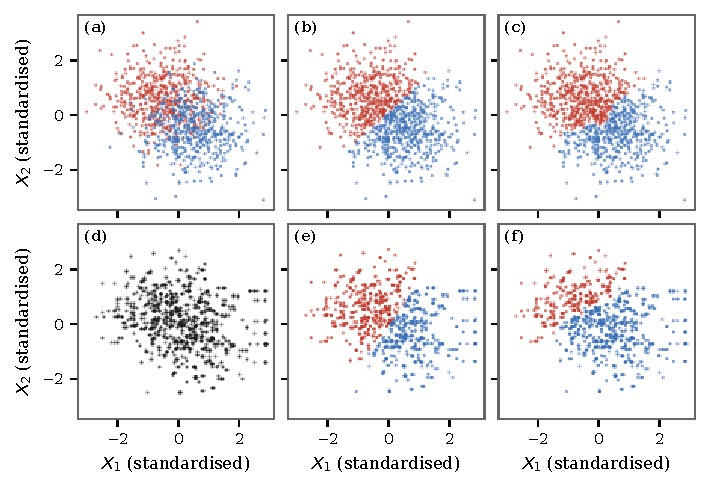
\includegraphics{figures/fig_normal.pdf}
\caption{Normal (spherical) components: geometry largely preserved under
  synthesis. Top row, original data: (a) true group labels, (b) $k$-means
  partition, (c) Ward partition. Bottom row, the corresponding CART synthetic
  dataset: (d) synthetic group label, (e) $k$-means partition, (f) Ward
  partition. The data shown are replicate 1 of the scenario $k = 2$, $p = 2$,
  $\rho = 0$, $\sigma = 2$ and its first synthetic draw; axes are the two
  standardised features. In the partition panels, colours are matched across
  rows by Hungarian alignment, so the same colour denotes corresponding groups
  in the original and synthetic panels. Panel (d) is drawn in a single colour:
  the group label in the synthetic data is itself synthesised, so it is a
  prediction from the synthetic features rather than a planted truth, and it
  has no bijective correspondence with the original groups. Both rows contain
  the same number of observations ($N = 1000$); the synthetic panels can look
  sparser only because CART resamples observed values, so that points coincide
  more often.}
\label{fig:normal}
\end{figure}

\begin{figure}[t]
\centering
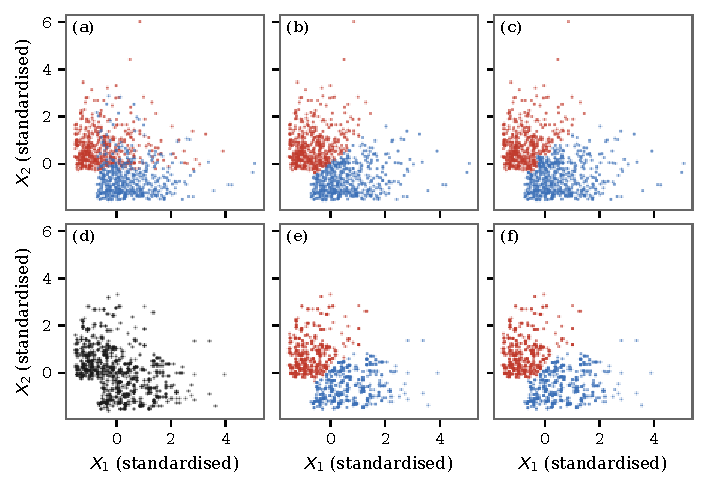
\includegraphics{figures/fig_gamma.pdf}
\caption{Gamma (right-skewed) components: the same synthesis mechanism breaks
  smooth tails into axis-aligned blocks. Panel layout (a)--(f), colour
  matching, the single-colour panel (d), the replicate and draw shown, and the
  scenario ($k = 2$, $p = 2$, $\rho = 0$, $\sigma = 2$) are as in
  Fig.~\ref{fig:normal}, and both rows again contain $N = 1000$ observations.
  Comparing panel (d) with panel (a) shows the artefact directly: the
  continuous density gradient of the original becomes a set of discrete
  rectangular patches.}
\label{fig:gamma}
\end{figure}

\subsection{Number of groups}
\label{sec:count}

The number of clusters estimated from synthetic data can be evaluated against
two references, each addressing a different question
(Section~\ref{sec:metrics}). Comparison with the planted number of groups
($\mathrm{RR}$) assesses whether the synthetic data support recovery of the
underlying truth, and so combines synthesis distortion with the inability of
the clustering procedure to find the planted structure at all. Comparison with
the number estimated from the original data ($\mathrm{AG}$) removes the second
component but retains the ordinary resampling instability of $\hat{k}$, which
the bootstrap null measures (Section~\ref{sec:excess}). Both references are
reported throughout, and Figure~\ref{fig:recovery} shows each against
separation, stratified by the true number of groups.

Separation is the decisive factor under both references. Against the planted
number of groups, recovery rises from $0.247$ ($k$-means) and $0.281$ (Ward)
at $\sigma = 0.1$, through $0.288$ and $0.295$ at $\sigma = 2$, to $0.810$ and
$0.789$ at $\sigma = 6$ and $0.954$ and $0.950$ at $\sigma = 10$. The
transition is sharp: up to $\sigma = 2$ recovery is low and dominated by the
overlap of the groups themselves, while at $\sigma = 10$ it is high for every
$k$.

Against the number estimated from the original data the picture is markedly
more favourable, and the gap is largest exactly where the groups overlap:
agreement is $0.684$ ($k$-means) and $0.646$ (Ward) at $\sigma = 0.1$, rising
to $0.982$ and $0.975$ at $\sigma = 10$, for overall agreement of $0.839$ and
$0.811$. The explanation is that at low separation the algorithms frequently
fail to recover the planted count from the original data as well: at
$\sigma = 0.1$, $k$-means finds the true $k$ in only $0.233$ of original
datasets and Ward in $0.294$. Much of what the first reference records as a
failure of synthesis is therefore a failure of clustering under overlap, which
synthesis reproduces.

The number of groups behaves very differently under the two references.
Against the planted count, recovery is much higher for fewer groups: $0.819$
for $k$-means at $k = 2$, against $0.468$ at $k = 3$ and $0.437$ at $k = 4$;
in the overlapping regime the three- and four-group cases are almost never
recovered (at most $0.12$), yet they exceed $0.90$ once $\sigma = 10$. Against
the original data, this pattern largely disappears ($0.847$, $0.838$ and
$0.833$). The difficulty of larger $k$ thus lies mainly in the clustering
problem, which synthesis reproduces, rather than in synthesis itself. The
partial $\eta^2$ values from the main-effects model make the contrast
explicit: for the planted reference, separation ($0.565$ for $k$-means,
$0.577$ for Ward) and $k$ ($0.287$ and $0.357$) dominate, whereas for
agreement with the original data separation ($0.245$ and $0.229$) is followed
by correlation ($0.141$ and $0.075$) and distribution family ($0.019$ and
$0.105$), with $k$ below $0.001$. For agreement, however, the main effects
explain only a third of the variation ($R^2 = 0.340$ and $0.349$); adding all
two-way interactions raises $R^2$ to $0.606$ and $0.605$, with large
correlation-by-separation terms ($0.282$ and $0.179$), so the ranking
describes average tendencies rather than a separable structure.
Table~\ref{tab:factors} reports the marginal means for every design factor
under both references.

\begin{figure}[t]
\centering
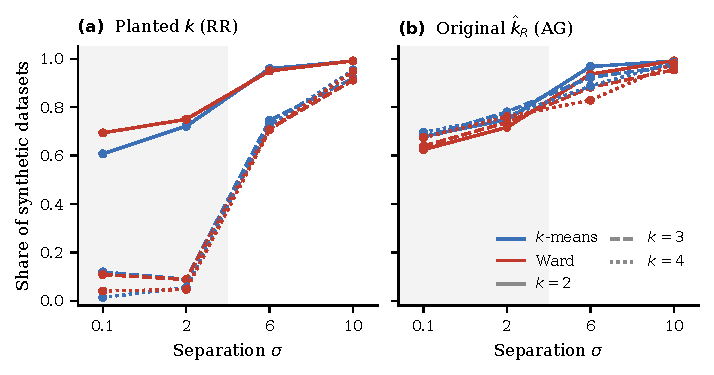
\includegraphics{figures/fig_recovery.pdf}
\caption{Cluster-count agreement between synthetic and original data, against
  separation and stratified by the true number of groups, under two reference
  conventions: (a) agreement with the number of groups planted by the
  simulation ($\mathrm{RR}$); (b) agreement with the number the same
  algorithm recovers from the original data ($\mathrm{AG}$). The separation
  levels are shown as categories because they are not equally spaced; the
  shaded region marks overlapping groups ($\sigma \le 2$). In (a), agreement is
  low while the groups overlap for $k \ge 3$ and moderate for $k = 2$; (b)
  stays higher throughout and depends far less on $k$, because in the
  overlapping regime the algorithms often fail to recover the planted count
  from the original data as well. Candidate range $\{2,\dots,8\}$; each point
  pools 60{,}000 original--synthetic pairs.}
\label{fig:recovery}
\end{figure}

\begin{table}[!tbp]
\centering
\caption{Agreement in the number of groups by design factor, over the full
         720{,}000-evaluation design, under the two references of
         Eq.~\eqref{eq:sr}: the planted number of groups ($\mathrm{RR}$) and
         the number estimated from the original data ($\mathrm{AG}$). Each
         entry is a marginal mean over all other factors; candidate range
         $\{2,\dots,8\}$. Wilcoxon $p$: paired signed-rank test of $k$-means
         against Ward across the 144 scenario-level means. The capped range
         $\{2,\dots,\min(k+3,8)\}$ is reported in Supplementary Table~S2.}
\label{tab:factors}
\small
\begin{tabular}{llrrrr}
\toprule
 & & \multicolumn{2}{c}{Planted $k$ (RR)} & \multicolumn{2}{c}{Original $\hat{k}_R$ (AG)} \\
\cmidrule(lr){3-4}\cmidrule(lr){5-6}
Factor & Level & $k$-means & Ward & $k$-means & Ward \\
\midrule
Separation $\sigma$ & $0.1$\textsuperscript{a} & 0.247 & 0.281 & 0.684 & 0.646 \\
 & $2$\textsuperscript{a} & 0.288 & 0.295 & 0.764 & 0.738 \\
 & $6$ & 0.810 & 0.789 & 0.926 & 0.882 \\
 & $10$ & 0.954 & 0.950 & 0.982 & 0.975 \\
\addlinespace
Number of groups $k$ & $2$ & 0.819 & 0.846 & 0.847 & 0.817 \\
 & $3$ & 0.468 & 0.455 & 0.838 & 0.803 \\
 & $4$ & 0.437 & 0.435 & 0.833 & 0.811 \\
\addlinespace
Dimensionality $p$ & $2$ & 0.605 & 0.613 & 0.817 & 0.756 \\
 & $5$ & 0.554 & 0.563 & 0.849 & 0.806 \\
 & $10$ & 0.565 & 0.560 & 0.851 & 0.870 \\
\addlinespace
Correlation $\rho$ & $0$ & 0.553 & 0.567 & 0.753 & 0.744 \\
 & $0.4$ & 0.597 & 0.590 & 0.925 & 0.877 \\
\addlinespace
Distribution $F$ & Normal & 0.593 & 0.604 & 0.869 & 0.890 \\
 & Gamma & 0.557 & 0.554 & 0.809 & 0.731 \\
\midrule
Overall & & 0.575 & 0.579 & 0.839 & 0.811 \\
Wilcoxon $p$ & & \multicolumn{2}{c}{0.750} & \multicolumn{2}{c}{$5.4\times10^{-5}$} \\
\bottomrule
\end{tabular}

\par\smallskip
\begin{minipage}{0.92\linewidth}\footnotesize
\textsuperscript{a}All collapse cells lie at $\sigma \le 2$: scenarios with
$k \ge 3$ in which every original dataset gives $\hat{k}_R = 2$ (22 of 96 for
$k$-means, 26 of 96 for Ward). They contain $15.3\%$ and $18.1\%$ of all
evaluations, and agreement is $0.955$ and $0.929$ inside them against $0.799$
and $0.762$ outside (Supplementary Section~S6).
\end{minipage}
\end{table}

Three further patterns in Table~\ref{tab:factors} deserve comment. First,
agreement with the original data is higher for correlated components
($0.925$ versus $0.753$ for $k$-means; $0.877$ versus $0.744$ for Ward), but
this is an effect of the estimator rather than of synthesis. At
$\sigma \le 2$ the silhouette scan returns $\hat{k}_R = 2$ for $91.1\%$
($k$-means) and $87.8\%$ (Ward) of original datasets with $\rho = 0.4$,
against $38.3\%$ and $62.2\%$ with $\rho = 0$, so original and synthetic
estimates coincide largely because both collapse onto the smallest candidate.
Where the estimator is not collapsed ($\sigma \ge 6$), agreement is slightly
lower for correlated components ($0.948$ versus $0.960$ for $k$-means;
$0.914$ versus $0.944$ for Ward). Second, dimensionality has opposite effects
in the two regimes. At $\sigma \le 2$ Ward's agreement rises with $p$ ($0.536$,
$0.703$ and $0.839$ at $p = 2$, $5$ and $10$), again because of collapse: at
$p = 10$ and $\sigma \le 2$ the scan selects $\hat{k}_R = 2$ for $80.8\%$
($k$-means) and $90.0\%$ (Ward) of original datasets. At $\sigma = 6$, where
the groups are separated but not trivially so, agreement falls with $p$
($k$-means $0.976$, $0.903$ and $0.899$; Ward $0.976$, $0.853$ and $0.818$).
Third, the collapse cells marked in Table~\ref{tab:factors}, a sixth of the
design, contribute near-automatic agreement and raise the overall values. The
distribution family produces a consistent gap under both references, which
Section~\ref{sec:distribution} examines.

\subsection{Agreement relative to the bootstrap null}
\label{sec:excess}

Table~\ref{tab:null} sets $\mathrm{AG}$ beside its bootstrap null. Both
algorithms agree with the original estimate less often after synthesis than
after bootstrap resampling: overall $\mathrm{AG}_0$ is $0.871$ for $k$-means
and $0.826$ for Ward, so the excess is $-0.032$ and $-0.016$. Synthetic
agreement lies below the null in 99 of the 144 scenarios for $k$-means
(10 above, 35 ties; Wilcoxon $p = 1.1 \times 10^{-11}$) and in 90 for Ward
(30 above, 24 ties; $p = 4.8 \times 10^{-6}$). The loss attributable to CART
beyond resampling is therefore real but small, a few points of agreement,
against a resampling instability that is already sizeable: even a bootstrap
resample of the original fails to reproduce $\hat{k}_R$ in $12.9\%$ of cases
for $k$-means and $17.4\%$ for Ward. Two independent original datasets
from the same scenario, a coarser reference that also changes the centroid
geometry, agree in $0.801$ and $0.767$ of pairs (Supplementary Section~S4).

\begin{table}[!tbp]
\centering
\caption{Agreement with the original estimate after CART synthesis
         ($\mathrm{AG}$) and after bootstrap resampling of the original data
         ($\mathrm{AG}_0$, $B = 30$ resamples per original dataset), and the
         excess $\mathrm{AG} - \mathrm{AG}_0$; negative values mean that
         synthesis loses agreement beyond resampling. Candidate range
         $\{2,\dots,8\}$. The excess is computed before rounding.}
\label{tab:null}
\small
\begin{tabular}{llrrrrrr}
\toprule
 & & \multicolumn{3}{c}{$k$-means} & \multicolumn{3}{c}{Ward} \\
\cmidrule(lr){3-5}\cmidrule(lr){6-8}
Stratum & Level & AG & AG$_0$ & Excess & AG & AG$_0$ & Excess \\
\midrule
Separation $\sigma$ & $0.1$ & 0.684 & 0.721 & $-0.038$ & 0.646 & 0.644 & $+0.002$ \\
 & $2$ & 0.764 & 0.814 & $-0.051$ & 0.738 & 0.754 & $-0.016$ \\
 & $6$ & 0.926 & 0.960 & $-0.034$ & 0.882 & 0.923 & $-0.040$ \\
 & $10$ & 0.982 & 0.989 & $-0.007$ & 0.975 & 0.984 & $-0.009$ \\
\addlinespace
Distribution $F$ & Normal & 0.869 & 0.880 & $-0.011$ & 0.890 & 0.902 & $-0.012$ \\
 & Gamma & 0.809 & 0.863 & $-0.053$ & 0.731 & 0.750 & $-0.020$ \\
\addlinespace
Normal, $\sigma$ & $0.1$ & 0.665 & 0.655 & $+0.011$ & 0.782 & 0.773 & $+0.009$ \\
 & $2$ & 0.879 & 0.903 & $-0.024$ & 0.873 & 0.886 & $-0.013$ \\
 & $6$ & 0.947 & 0.974 & $-0.028$ & 0.924 & 0.964 & $-0.040$ \\
 & $10$ & 0.983 & 0.988 & $-0.005$ & 0.982 & 0.986 & $-0.004$ \\
\addlinespace
Gamma, $\sigma$ & $0.1$ & 0.702 & 0.788 & $-0.086$ & 0.511 & 0.515 & $-0.004$ \\
 & $2$ & 0.648 & 0.726 & $-0.078$ & 0.603 & 0.623 & $-0.019$ \\
 & $6$ & 0.906 & 0.946 & $-0.040$ & 0.841 & 0.881 & $-0.041$ \\
 & $10$ & 0.981 & 0.991 & $-0.010$ & 0.969 & 0.983 & $-0.014$ \\
\midrule
Overall &  & 0.839 & 0.871 & $-0.032$ & 0.811 & 0.826 & $-0.016$ \\
\bottomrule
\end{tabular}

\end{table}

\subsection{Geometric fidelity}
\label{sec:geometry}

Figure~\ref{fig:fidelity} traces the geometric-fidelity metrics against
separation, together with their bootstrap floors, and
Table~\ref{tab:floor} summarises them. Mean centroid distance falls steeply as
groups separate, from $0.604$ ($k$-means) and $0.859$ (Ward) at
$\sigma = 0.1$ to $0.090$ and $0.095$ at $\sigma = 10$, and mean variance
difference falls from $0.353$ and $0.613$ to $0.112$ and $0.133$. Observed
values are lower for $k$-means in 133 of the 144 scenarios for MCD, in all 144
for MVD and in 138 for $\Delta G$ (paired Wilcoxon $p < 10^{-20}$ for each).

Most of this distortion, however, is already produced by resampling.
Bootstrap resampling alone reproduces $0.222$ of the $0.303$ observed MCD for
$k$-means and $0.403$ of $0.460$ for Ward, $0.150$ of $0.219$ and $0.324$ of
$0.392$ for MVD, and $0.021$ of $0.030$ and $0.053$ of $0.061$ for $\Delta G$,
and the floor already places $k$-means below Ward (in 121, 135 and 132 of the
144 scenarios for MCD, MVD and $\Delta G$). CART adds a positive excess in
almost every scenario (MCD 144 and 143 of 144 for $k$-means and Ward; MVD 144
and 141; $\Delta G$ 144 and 129; $p < 10^{-20}$ for each), but the excess is
not smaller for $k$-means: it is larger for MCD ($0.081$ versus $0.057$;
Wilcoxon $p = 8.8 \times 10^{-6}$) and equal for MVD ($0.069$ versus $0.068$; $p = 0.973$) and nearly equal for
$\Delta G$ ($0.009$ versus $0.008$; $p = 0.462$, but $p = 0.002$ at $n = 50$). The
lower geometric distortion of $k$-means on synthetic data is therefore
inherited from its lower distortion under resampling, not produced by a
smaller effect of CART.

The scale-free metrics correct the reading of the separation trend. In units
of the within-component standard deviation, the centroid displacement still
falls with separation ($k$-means $0.605$ to $0.189$; Ward $0.860$ to $0.201$),
and CART moves the centroids by about $0.10$ ($k$-means) and $0.08$ (Ward)
within-component standard deviations beyond resampling. Dispersion behaves
differently. The relative variance difference shows that a synthetic
cluster's dispersion deviates from the original's by $8.2\%$ on average for
$k$-means and $15.2\%$ for Ward, of which $5.5$ and $12.6$ points are
resampling; the excess attributable to CART is about $2.7$ points for both
($0.027$ versus $0.026$; $p = 0.891$). This excess does not decline with
separation; it grows ($k$-means $0.022$, $0.021$, $0.030$ and $0.035$ across
the four levels of $\sigma$; Ward $0.015$, $0.013$, $0.036$ and $0.041$). The
decline of absolute MVD with $\sigma$ is thus mostly a decline of the floor
and a change of units, not a reduction of the dispersion distortion that CART
introduces.

\begin{figure}[t]
\centering
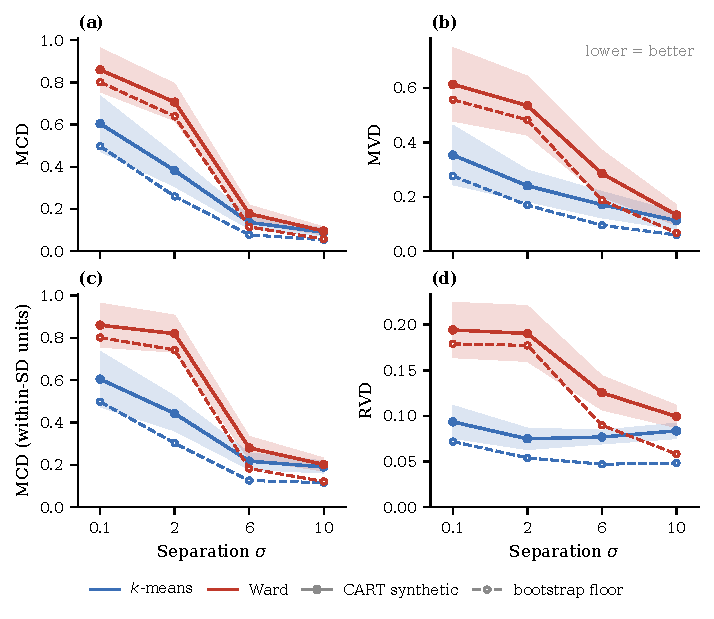
\includegraphics{figures/fig_fidelity.pdf}
\caption{Geometric fidelity against separation, observed after CART synthesis
  (solid lines, filled markers) and under bootstrap resampling of the original
  data (dashed lines, open markers; $B = 30$). (a) Mean centroid distance and
  (b) mean variance difference, in the units of the scaler fit on the
  original data; (c) mean centroid distance in units of the within-component
  standard deviation ($\mathrm{MCD}_{\mathrm{sd}}$); (d) relative variance
  difference (RVD). Points are means of the 36 scenario-level means at each
  separation level; bands are $\pm 1.96$ standard errors across those
  scenarios and describe the spread over the design, not sampling
  uncertainty. The vertical distance between a solid and a dashed line of the
  same colour is the excess attributable to CART.}
\label{fig:fidelity}
\end{figure}

\begin{table}[!tbp]
\centering
\caption{Geometric fidelity after CART synthesis (observed), under bootstrap
         resampling of the original data (floor, $B = 30$) and their
         difference (excess), averaged over the 144 scenario means, at the
         planted $k$. MCD, MVD and $\Delta G$ are in the units of the scaler
         fit on the original data; $\mathrm{MCD}_{\mathrm{sd}}$ is in
         within-component standard deviations and RVD is a relative error.
         Last column: Wilcoxon $p$ for the excess of $k$-means against the
         excess of Ward across the 144 scenarios. Values by separation,
         distribution family and dimensionality are in Supplementary
         Section~S5.}
\label{tab:floor}
\small
\begin{tabular}{lrrrrrrr}
\toprule
 & \multicolumn{3}{c}{$k$-means} & \multicolumn{3}{c}{Ward} & Excess \\
\cmidrule(lr){2-4}\cmidrule(lr){5-7}
Metric & Observed & Floor & Excess & Observed & Floor & Excess & $p$ \\
\midrule
MCD & 0.303 & 0.222 & 0.081 & 0.460 & 0.403 & 0.057 & $8.8\times10^{-6}$ \\
MVD & 0.219 & 0.150 & 0.069 & 0.392 & 0.324 & 0.068 & 0.973 \\
$\Delta G$ & 0.030 & 0.021 & 0.009 & 0.061 & 0.053 & 0.008 & 0.462 \\
\addlinespace
MCD$_{\mathrm{sd}}$ & 0.363 & 0.260 & 0.103 & 0.540 & 0.462 & 0.078 & $2.7\times10^{-5}$ \\
RVD & 0.082 & 0.055 & 0.027 & 0.152 & 0.126 & 0.026 & 0.891 \\
\bottomrule
\end{tabular}

\end{table}

Total dispersion distortion grows with dimensionality (Supplementary
Fig.~S3a): MVD rises from $0.06$ at $p = 2$ to $0.39$ at $p = 10$ for $k$-means
and from $0.13$ to $0.65$ for Ward. Because $v_j$ in Eq.~\eqref{eq:mvd} sums
squared deviations over the $p$ coordinates, $\mathrm{MVD}/p$ is roughly
constant ($k$-means $0.032$, $0.040$ and $0.039$ at $p = 2, 5, 10$; Ward
$0.067$, $0.078$ and $0.065$) and the floor grows in the same way, so much of
the accumulation is resampling noise summed over coordinates; the
per-coordinate excess attributable to CART increases only mildly with $p$
($k$-means $0.008$, $0.011$ and $0.013$; Ward $0.006$, $0.010$ and $0.014$).

Group balance is better preserved on Normal than on Gamma data (Supplementary
Fig.~S3b; $\Delta G$ $0.028$ versus $0.032$ for $k$-means, $0.057$ versus
$0.065$ for Ward). $k$-means yields lower $\Delta G$ than Ward (in 138 of 144
scenarios; $0.030$ versus $0.061$), but the floor shows the same ordering
($0.021$ versus $0.053$): with equal planted group sizes, the cluster sizes of
a $k$-means partition fluctuate less under resampling, and hence under
synthesis, consistent with the tendency of the $k$-means criterion to produce
clusters of similar size \citep{xiong2009}. Whether $k$-means would understate
a genuine size imbalance is left to future work (Section~\ref{sec:future}).

\subsection{Distribution family}
\label{sec:distribution}

The distribution family is the factor that exposes the CART artefact most
directly. Figure~\ref{fig:distribution} stratifies count agreement by
distribution and separation under both references, each shown with its
reference on data without synthesis. Against the planted number of groups
(panels a and b), the two families show similar recovery while the groups
overlap and diverge at intermediate separation: at $\sigma = 6$, $k$-means
recovers the planted count $86.2\%$ of the time for Normal data but only
$75.9\%$ for Gamma data (Ward: $84.5\%$ versus $73.2\%$). Almost all of this
gap, however, is already present in the original data, where the planted
count is recovered in $90.0\%$ versus $80.0\%$ of datasets ($k$-means; Ward
$91.1\%$ versus $78.9\%$). It therefore reflects mainly how difficult skewed
groups are to cluster, not what synthesis does to them.

Against the original data (panels c and d), the Gamma penalty is concentrated
where the groups overlap and is much larger for Ward. At $\sigma = 0.1$,
Ward's agreement is $0.782$ for Normal but only $0.511$ for Gamma data, and at
$\sigma = 2$ it is $0.873$ versus $0.603$; the corresponding values for
$k$-means are $0.665$ versus $0.702$ and $0.879$ versus $0.648$. At
$\sigma = 6$ the gap narrows ($k$-means $0.947$ versus $0.906$; Ward $0.924$
versus $0.841$), and at $\sigma = 10$ a small gap remains for Ward ($0.982$
versus $0.969$; $k$-means $0.983$ versus $0.981$). The bootstrap null shows
where this penalty comes from. For Ward, the null already contains it:
$\mathrm{AG}_0$ is $0.515$ for Gamma and $0.773$ for Normal data at
$\sigma = 0.1$, so the low agreement of Ward on skewed, overlapping data is an
instability of its silhouette estimate that synthesis inherits, and the
Gamma excess is small at every separation (between $-0.041$ and $-0.004$). For
$k$-means the null is higher on Gamma data ($0.788$ at $\sigma = 0.1$ and
$0.726$ at $\sigma = 2$), and the loss attributable to CART is largest exactly
there ($-0.086$ and $-0.078$).

This addresses the first objective. CART preserves the structure needed to
recover the number of groups on Normal data to within about one point of the
bootstrap null (excess $-0.011$ for $k$-means and $-0.012$ for Ward), and its
hardening of skewed densities lowers agreement on Gamma data beyond
resampling, most markedly for $k$-means when groups overlap. The larger Gamma
penalty seen for Ward in the raw agreement is mainly the instability of its
estimate on skewed, overlapping data rather than a larger effect of CART.

\begin{figure}[t]
\centering
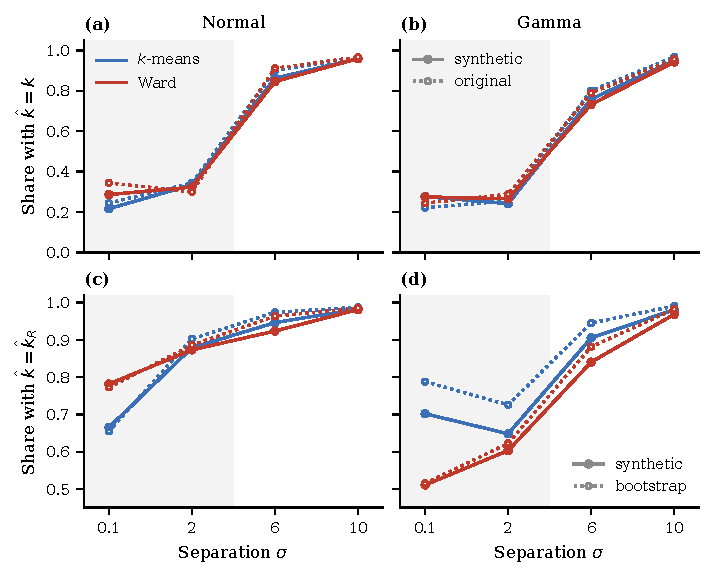
\includegraphics{figures/fig_distribution.pdf}
\caption{Cluster-count agreement by distribution family (columns: Normal,
  Gamma) and separation, under the two references (candidate range
  $\{2,\dots,8\}$). (a, b) Share of synthetic datasets with
  $\hat{k}_S = k$ (RR; solid) beside the share of original datasets with
  $\hat{k}_R = k$ (dotted, open markers). (c, d) Share of synthetic datasets
  with $\hat{k}_S = \hat{k}_R$ (AG; solid) beside the share of bootstrap
  resamples with $\hat{k}_b = \hat{k}_R$ ($\mathrm{AG}_0$; dotted, open
  markers). The vertical distance between a solid and a dotted line of the
  same colour is the part of the disagreement attributable to CART. Separation
  is shown as a categorical axis; the shaded region marks $\sigma \le 2$.}
\label{fig:distribution}
\end{figure}

\subsection{Agreement between the two algorithms}
\label{sec:algo}

Whether the two methods differ in robustness to synthetic distortion was the
third objective, and the answer depends on the reference. Against the planted
number of groups the two are indistinguishable: overall recovery is $0.575$
for $k$-means and $0.579$ for Ward, a paired Wilcoxon signed-rank test across
the 144 scenario-level means finds no significant difference ($W = 3508.5$,
$p = 0.750$), and the two algorithms reach the same outcome in $92.0\%$ of
individual evaluations.

Against the original data, $k$-means reproduces the number of groups more
often than Ward: overall agreement is $0.839$ versus $0.811$, $k$-means is
higher in 90 of the 144 scenarios (30 lower, 24 ties), and the paired test is
significant ($W = 2088.5$, $p = 5.4 \times 10^{-5}$). For an analyst who will
cluster a synthetic release, this is the practically relevant comparison, and
it is not uniform. The advantage of $k$-means arises on Gamma data ($0.809$
versus $0.731$; higher in 59 of 72 scenarios, $p = 2.6 \times 10^{-6}$),
where it is significant at $\sigma = 0.1$ ($0.702$ versus $0.511$,
$p = 0.002$), $\sigma = 6$ ($0.906$ versus $0.841$, $p = 0.001$) and
$\sigma = 10$ ($0.981$ versus $0.969$, $p = 0.006$) but not at $\sigma = 2$
($0.648$ versus $0.603$, $p = 0.099$). On Normal data there is no difference
($0.869$ versus $0.890$, $p = 0.595$), and in the most overlapping Normal
scenarios Ward is numerically higher ($0.782$ versus $0.665$ at
$\sigma = 0.1$; $p = 0.136$). The conclusion is unchanged under the capped
candidate range (Supplementary Section~S3).

The bootstrap null shows why. The same advantage is already present without
synthesis: $\mathrm{AG}_0$ is $0.871$ for $k$-means against $0.826$ for Ward
($W = 966$, $p = 6.0 \times 10^{-5}$), and $0.863$ against $0.750$ on Gamma
data ($p = 6.3 \times 10^{-7}$), while on Normal data the nulls do not differ
($0.880$ versus $0.902$, $p = 0.900$). The silhouette-based estimate of $k$ is
more stable under resampling for $k$-means, particularly on skewed data, and
synthesis inherits that stability. Beyond resampling, $k$-means loses slightly
more agreement than Ward (difference in excess $-0.017$, $W = 2846$,
$p = 0.040$), again only on Gamma data ($-0.034$, $p = 0.024$; concentrated at
$\sigma = 0.1$, $-0.082$, and $\sigma = 2$, $-0.058$), with no difference on Normal data ($p = 0.640$). A replication with $n = 50$
original datasets per scenario gives the same difference with much stronger
evidence ($-0.018$, $p = 1.2 \times 10^{-5}$; Supplementary Section~S12). The higher agreement of $k$-means on
synthetic data thus reflects the greater stability of its $\hat{k}$, not
smaller damage from CART, and the same holds for the geometric metrics
(Section~\ref{sec:geometry}).

As a complementary check on internal cohesion, the difference in mean
silhouette width between synthetic and original partitions at the planted $k$
is small and centred near zero at every separation (at most $0.0125$ in
absolute value, for Ward at $\sigma = 0.1$). The absolute levels are nearly
identical ($k$-means $0.396$ versus $0.397$; Ward $0.376$ versus $0.377$),
suggesting that the apparent clustering quality is similar before and after
synthesis. This is reassuring, but it also means that silhouette alone would
fail to flag the geometric distortions the other metrics detect, an
instructive negative result for anyone tempted to validate a synthetic release
with an internal index.

% =====================================================================
\section{Case study: the Reaven--Miller diabetes data}\label{sec:case}

To illustrate the conclusions from the simulation study, we apply the same
procedure to the diabetes data \citep{reaven1979}. The data comprise $145$
patients classified clinically as normal ($76$), chemical diabetes ($36$) or
overt diabetes ($33$). Following \citet{reaven1979}, we use three of the five
variables in the distributed data: the areas under the plasma glucose and
insulin curves during an oral glucose tolerance test, and the steady-state
plasma glucose (SSPG), taken from the copy of the data distributed with the
\textsf{R} package \texttt{rrcov} \citep{todorov2009}. The three variables are
right-skewed (skewness $1.8$, $1.8$ and $0.7$), and glucose area and SSPG are
strongly correlated ($r = 0.77$). As in the simulation, the data were
standardised with the means and standard deviations of the original, and
$m = 1000$ synthetic datasets were generated with the settings of the
simulation: CART with proper synthesis and a minimum leaf size of ten, with the
variables synthesised in the order glucose, insulin and SSPG and the clinical
class last. The bootstrap null used $B = 1000$ resamples of the original rows.
Uncertainty is Monte Carlo uncertainty over draws only (\textsf{R} 4.5.3,
\texttt{synthpop} 1.9.3, \texttt{rpart} 4.1.27; evaluation with the code of the
simulation). In the synthetic data the block artefact of
Figs.~\ref{fig:normal}--\ref{fig:gamma} appears as runs of repeated values and
empty bands (Fig.~\ref{fig:diabetes}a--b).

\citet{reaven1979} identified three groups, a central body and two wings in a
rotating PRIM-9 display, and a three-group nearest-mean clustering
\citep{friedman1967} reproduced the clinical classification closely ($84$,
$35$ and $26$ patients, with $20$ patients reassigned). There the number of
groups was fixed in advance; estimated from the data, as in our design, the
silhouette selects $\hat k = 2$ for both methods, but only by
a small margin over three groups (average silhouette width $0.571$ versus
$0.547$ for $k$-means, $0.567$ versus $0.544$ for Ward). The original data thus
sit close to the boundary between two and three groups, and the selected
$\hat k$ is expected to be unstable under any perturbation. This near tie
governs the synthetic results (Fig.~\ref{fig:diabetes}c): the synthetic data
reproduce $\hat k = 2$ in $62.9\%$ of draws for $k$-means and $63.2\%$ for Ward
(AG), and the two methods do not differ (exact McNemar test on the paired
draws, $58$ versus $61$ discordant draws, $p = 0.85$). Resampling the original
rows gives almost the same agreement ($\mathrm{AG}_0 = 0.667$ and $0.637$), so
the excess over the null is $-0.038$ for $k$-means and $-0.005$ for Ward (Monte
Carlo standard error $0.021$), neither distinguishable from zero.

The partition-level metrics use the clinical $k = 3$, the analogue of the
planted $k$ in the simulation. To measure whether the same patients are grouped
together without matching synthetic to original records, each synthetic dataset
is partitioned with $k = 3$, every original patient is assigned to the nearest
of its cluster means \citep{dudoit2002,tibshirani2005}, and the adjusted Rand
index (ARI; \citealp{hubert1985}) compares this assignment with the original
partition of the same $145$ patients. ARI is $1$ for identical partitions and
near $0$ for chance agreement; for Ward, whose partition is not a
nearest-centroid one, the ceiling is $0.955$, which the bootstrap null
includes.

All metrics show the same qualitative pattern as the simulation, with mostly
larger magnitudes (Table~\ref{tab:case}). Every geometric metric exceeds its
bootstrap floor for both methods by more than four Monte Carlo standard errors.
ARI is $0.856$ for $k$-means and $0.797$ for Ward, below its bootstrap null by
$0.066$ and $0.040$: synthesis also moves patients between groups beyond what
resampling does, as it does over the whole simulation ($0.036$ and $0.011$
below the null; Supplementary Section~S10). Against the clinical classes, the
original partitions give an ARI of $0.504$ ($k$-means) and $0.536$ (Ward), the
partitions transferred from the synthetic data $0.481$ and $0.471$, and those
from resamples $0.495$ and $0.480$: the synthetic data recover the diagnostic
groups slightly less well than a resample. As the clinical classes were defined
mainly from the glucose tolerance test, this comparison is partly circular.

As in the simulation, the count of groups is limited mainly by how stable
$\hat k$ is on the original data, while CART adds a measurable distortion of
the partition itself. The advantage of $k$-means in AG seen for skewed simulated
data does not appear here. This is consistent with its explanation: $k$-means
is only slightly more stable under resampling ($\mathrm{AG}_0$ $0.667$ versus
$0.637$; exact McNemar test on the paired resamples, $86$ versus $56$
discordant, $p = 0.015$), and synthesis removes that margin (AG $0.629$ versus
$0.632$). In all six orders of the three variables
(Supplementary Section~S11) every geometric excess is positive, every ARI
excess negative and the AG of the two methods within $0.05$; count agreement
falls furthest below its null when glucose area is synthesised last (AG excess
down to $-0.12$ for $k$-means and $-0.14$ for Ward).

\begin{figure}[t]
\centering
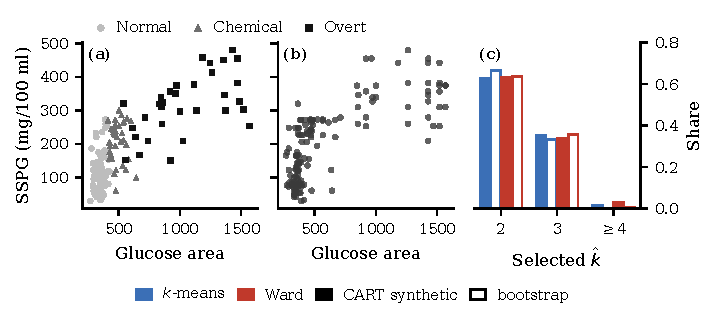
\includegraphics{figures/fig_diabetes.pdf}
\caption{Diabetes data, $N = 145$. (a) Original data by clinical class.
(b) One CART synthetic dataset (single colour, as in
Figs.~\ref{fig:normal}--\ref{fig:gamma}). (c) Silhouette-selected $\hat k$
over $m = 1000$ synthetic datasets (filled) and $B = 1000$ bootstrap resamples
(open); on the original data both methods select $\hat k = 2$.}
\label{fig:diabetes}
\end{figure}

\begin{table}[!tbp]
\centering
\caption{Diabetes case study: means over $m = 1000$ synthetic datasets and
  $B = 1000$ bootstrap resamples, and the excess (synthetic minus bootstrap).
  AG uses $\hat k$, the other metrics $k = 3$; ARI (clinical) compares the
  transferred partition with the clinical classes. Monte Carlo standard errors
  of the excess: $0.021$ for AG, $0.002$--$0.010$ otherwise.}
\label{tab:case}
\small
\begin{tabular}{lrrrrrr}
\toprule
 & \multicolumn{3}{c}{$k$-means} & \multicolumn{3}{c}{Ward} \\
\cmidrule(lr){2-4}\cmidrule(lr){5-7}
Metric & Synthetic & Bootstrap & Excess & Synthetic & Bootstrap & Excess \\
\midrule
AG & 0.629 & 0.667 & $-$0.038 & 0.632 & 0.637 & $-$0.005 \\
ARI & 0.856 & 0.922 & $-$0.066 & 0.797 & 0.837 & $-$0.040 \\
\addlinespace
MCD & 0.383 & 0.229 & 0.154 & 0.472 & 0.348 & 0.124 \\
MVD & 0.216 & 0.165 & 0.051 & 0.313 & 0.242 & 0.070 \\
$\Delta G$ & 0.062 & 0.042 & 0.019 & 0.084 & 0.073 & 0.011 \\
RVD & 0.208 & 0.150 & 0.058 & 0.305 & 0.235 & 0.070 \\
\addlinespace
ARI (clinical) & 0.481 & 0.495 & $-$0.014 & 0.471 & 0.480 & $-$0.009 \\
\bottomrule
\end{tabular}

\end{table}

% =====================================================================
\section{Discussion}
% =====================================================================

This study evaluated whether CART-generated synthetic data preserve the
structural properties that cluster analysis relies on, comparing $k$-means and
Ward's hierarchical clustering across a 144-scenario factorial design and
720{,}000 synthetic-versus-original evaluations, each read against a bootstrap
resample of the same original data. Four findings emerge.

First, separation dominates agreement in the number of groups. Agreement with
the original data rises from $0.684$ ($k$-means) and $0.646$ (Ward) when the
groups overlap to $0.982$ and $0.975$ when they are well separated, and
recovery of the planted count rises from $0.247$ and $0.281$ to $0.954$ and
$0.950$. The number
of groups strongly affects recovery of the planted count ($0.819$ at $k = 2$
against $0.468$ and $0.437$ at $k = 3$ and $4$, for $k$-means) but has little
effect on agreement between original and synthetic estimates. Most of the
effect of $k$ is a property of the clustering problem that synthesis
reproduces rather than a distortion that synthesis introduces. Where groups
overlap, a sixth of the design consists of collapse cells in which the
silhouette scan returns two groups for every original dataset, and agreement
there is close to automatic.

Second, for a researcher who clusters a synthetic release, $k$-means
reproduces the number of groups found in the original data more often than
Ward's linkage ($0.839$ versus $0.811$). This happens on skewed Gamma data
($0.809$ versus $0.731$), at every separation except $\sigma = 2$, and not on
Normal data ($0.869$ versus $0.890$). The bootstrap null shows that this
advantage reflects the greater stability of the $k$-means estimate of $k$
under resampling ($\mathrm{AG}_0$ $0.871$ versus $0.826$), not smaller damage
from CART: the agreement lost to synthesis beyond resampling is small for
both methods ($0.032$ and $0.016$) and, if anything, slightly larger for
$k$-means. The geometry tells the same story. $k$-means shows lower centroid,
dispersion and cluster-size distortion on synthetic data, but most of each
metric is reproduced by resampling alone, and the excess attributable to CART
is not smaller for $k$-means (larger for MCD, equal or nearly equal for MVD, $\Delta G$ and RVD). For an applied analyst, the practical implication is that the choice of
algorithm matters more for the fidelity of a synthetic-data analysis than
accuracy against a ground truth would suggest, and that the reason is the
stability of the estimator rather than the generator.

Third, CART is not utility-neutral, and its effect depends on the underlying
distribution. On Normal data the count agreement after synthesis is within
about one point of the bootstrap null; on skewed Gamma data CART hardens smooth
density gradients into axis-aligned blocks, visibly distorting geometry and
lowering agreement beyond resampling, most for $k$-means when groups overlap.
CART adds a positive excess over the resampling floor to every geometric
metric in almost every scenario; in relative terms it changes within-cluster
dispersion by about $2.7\%$ beyond resampling, and this relative excess grows
rather than shrinks with separation.

Fourth, and methodologically, neither an internal validity index nor raw
agreement is a sufficient check. Silhouette values remain almost unchanged
even where centroid and dispersion fidelity degrade. A practitioner who
validates a synthetic release by confirming that its silhouette profile
matches the original may conclude that structure is intact in precisely the
settings where this analysis shows it is not. Raw agreement, in turn, mixes
the effect of the generator with the instability of the estimator, and the
comparison between algorithms changes once each method is set against its own
resampling null. The planted truth, the natural choice in a simulation,
answers yet another question, and in this study it masked the difference
between the two algorithms.

An interesting corollary of the design is that clustering can be read in the
other direction, as an instrument rather than an object of study. Because a
partition responds to local density, separability and dispersion
simultaneously, the agreement between partitions recovered from original and
synthetic data functions as a sensitive summary of geometric resemblance, one
that reacts to distortions which marginal and bivariate checks may not detect.
We did not pursue this here, but the metrics of Section~\ref{sec:metrics} could
be repurposed as general-utility diagnostics rather than task-specific ones.

\subsection{Relation to previous work}

The study extends \blindalt{\citet{anon2025}}{\citet{chen2025}} in three ways: a second algorithm that
shares the criterion of $k$-means but optimises it differently, a skewed
distribution family that exposes tree-synthesis artefacts, and structural
metrics that compare partitions recovered from the original and synthetic
data. It should be distinguished from the cluster-based utility measure of
\citet{woo2009}, which clusters the merged original and masked records and
measures how well each cluster mixes the two sources; that measure uses
clustering as a device for general utility, whereas we ask whether a
clustering analysis of the release reproduces the analysis of the original.
The conclusion that CART is a reasonable default for well-behaved data but
degrades on skewed distributions is consistent with the broader
\texttt{synthpop} literature \citep{nowok2016,snoke2018}, and the qualitative
block artefact matches the known axis-aligned bias of sequential tree
synthesis. The finding that utility rankings depend on the downstream task
echoes benchmarking work in the health-records setting
\citep{yan2022,elemam2022}, where the same generator changes position depending
on which analysis is used to score it, and an applied study of wearable
physiological data in mental-health monitoring similarly found that the
clustering utility of \texttt{synthpop} releases depends on the synthesis
settings \citep{vidiella2025}. The lower stability of Ward's estimate under
resampling is consistent with, although not directly comparable to, the
classical perturbation experiments of \citet{milligan1980}, which found that
methods differ in their sensitivity to error perturbation. A parallel question
arises when values are missing rather than synthesised: \citet{aschenbruck2023}
evaluate how imputation strategies affect the clusters subsequently recovered
from mixed-type data, and reach a structurally similar conclusion, that the
imputation model and the clustering method interact and cannot be assessed in
isolation. Since CART underlies both sequential synthesis and widely used
non-parametric imputation, the two literatures are closer than their
vocabularies suggest.

The count-agreement measure AG is, in effect, a stability criterion. A long
line of work validates clusterings, and chooses their number, by asking how
reproducibly a partition is recovered when the data are perturbed: by
subsampling \citep{levine2001,benhur2002}, by prediction from one half of the
sample to the other \citep{dudoit2002,lange2004,tibshirani2005,wang2010}, or by
the bootstrap \citep{jain1987,hennig2007,fang2012}; \citet{luxburg2010} reviews
these ideas. A synthetic release is a perturbation of the same kind, except
that the synthesiser, not the analyst, produces it, so AG measures the
stability of $\hat{k}$ under synthesis. Two results from this literature
govern how AG should be read. First, stability is not correctness:
\citet{bendavid2006} show that stability is driven by the structure of the
clustering objective rather than by the true number of groups, so AG must be
read together with recovery of the planted $k$; the collapse cells of
Section~\ref{sec:count}, where agreement is high because the estimator
returns two groups regardless, are an instance. Second, agreement under
perturbation has no natural zero, because $\hat{k}$ is already variable on the
original data. We therefore calibrate AG against a bootstrap null, in the
spirit of resampling-based assessments of cluster structure
\citep{suzuki2006,maitra2012}: agreement that a bootstrap resample of the
original already fails to reach cannot be attributed to CART. In this study
the calibration changes the comparison between algorithms, because the
advantage of $k$-means in AG is matched by its advantage in $\mathrm{AG}_0$. On
the analysis side, the closest analogue is validation of a clustering on
independent data \citep{ullmann2022}; a synthetic dataset can be regarded as a
validation sample that the data holder is able to release.

\subsection{Limitations}
\label{sec:limitations}

The evaluation rests on controlled simulations with known ground truth,
complemented by a single small real dataset (Section~\ref{sec:case}), and its
conclusions are scoped to the grid studied: correlations up
to $\rho = 0.4$, a single Gamma shape, $N = 1000$ and exactly equal group
sizes. This isolates mechanisms cleanly but limits direct generalisation to
data with missingness, mixed types, unequal group sizes and unknown
data-generating processes. The generator is limited to CART with a single
parameterisation (minimum leaf size ten, fixed variable order) and the
algorithms to $k$-means and Ward. Sample size was fixed at $N = 1000$ in the
simulation, so small-sample behaviour is examined only through the case study
($N = 145$). The number of groups is selected by the
silhouette criterion over $\hat{k} \ge 2$, so a single-cluster solution can
never be chosen, even when the groups overlap so strongly that one cluster is
the most reasonable description; other selection rules \citep{milligan1985}
may respond differently to synthesis. Count agreement is inflated where the
estimator collapses onto the smallest candidate, as happens at low $\sigma$,
high $p$ and $\rho = 0.4$, and should be read together with the bootstrap null
and the geometric metrics. The bootstrap null rests on $B = 30$ resamples per
original dataset, so comparisons of small excesses between the algorithms
carry Monte Carlo error; a replication with ten times as many original datasets
confirms them (Supplementary Section~S12). Every $k$-means fit uses the same seed; a check with
independent seeds (Section~\ref{sec:software}) showed no material effect. The Wilcoxon tests
and the $\pm 1.96$ standard-error bands are computed across the 144 scenarios
of a designed grid, so they compare methods over that grid rather than over a
population of scenarios.

Two conventions in the definition of MCD and MVD deserve emphasis, because both
affect the numbers themselves and not only their interpretation. The first is
what the metrics compare. Here they compare the partition recovered from the
original data against the partition recovered from the synthetic data, which is
the quantity a claim about synthesis requires; the superficially similar
practice of comparing a recovered partition against the planted labels of the
same dataset measures clustering accuracy instead, and carries no information
about the generator. The second is scale. Both metrics are computed after
standardising with a scaler fit on the pooled original data and applied
unchanged to the synthetic data, so both are expressed in units of the pooled
original feature scale. Standardising each dataset separately would rescale
away part of the distortion the metrics are meant to capture, but the common
scaler has its own dependence on the design: the pooled spread grows with
$\sigma$, so a standardised unit is a larger within-component distance at
large separation, and absolute MCD and MVD decline with $\sigma$ partly for
that reason. Neither convention is free of $\sigma$; only relative or
within-component versions are. We therefore report RVD and
$\mathrm{MCD}_{\mathrm{sd}}$ beside the absolute metrics, and read trends
across separation from them. Absolute values of MCD and MVD are not
comparable across studies that differ in either convention, and any
replication should state both explicitly. Both metrics are also unnormalised
sums over coordinates, so their absolute values grow with $p$ even at constant
per-coordinate distortion; comparisons across dimensionality should use
per-coordinate or relative versions.

\subsection{Future work}
\label{sec:future}

The central lesson generalises beyond the specific methods studied: synthetic
data utility is task-relative, and a generator that preserves marginal
resemblance need not preserve the higher-order geometry a clustering workflow
depends on. Practically, the results argue for validating structural fidelity
(distances, dispersion, separability, balance) against the intended analysis
and against a resampling reference, and for treating a clustering comparison
as a more demanding resemblance check than marginal summaries can provide.
Natural extensions include other synthesisers, such as conditional inference
trees \citep{hothorn2006}, CART with larger minimum leaf sizes, parametric
synthesisers, copulas and deep generative models; other clustering families,
in particular Gaussian mixture models with the number of components chosen by
BIC \citep{fraley2002,scrucca2016}, which can also return a single cluster, and
non-convex and density-based methods; unequal group sizes and stronger
correlations between features; varying $N$ to probe small-sample behaviour;
and a fuller study of the partition-level agreement introduced in the case
study, for example with transfer rules other than the nearest cluster mean. A promising direction
is to model the discrepancy $\Delta$ of Eq.~\eqref{eq:discrepancy} directly as
a learned function of the design factors, turning the utility surface itself
into a predictive tool.

As a concrete next step, we propose applying the same comparison to the
wearable dataset described in
\citet{vidiella2025}\blindhide{, to which we have direct access}. Beyond providing a second and larger real-data test of the present design, this dataset
would allow a comparison that neither study can perform alone. The present work
evaluates synthesis as substitution, in which the synthetic dataset replaces
the original. The applied study instead evaluates augmentation, in which the
synthetic records are appended to the real ones and the union is clustered.
These are different operations, and their effects are currently confounded
with sample size: doubling the number of observations alters neighbourhood
parameters and silhouette values independently of any distortion introduced by
the generator. A three-way comparison of the partitions recovered from the real
data, from the synthetic data alone, and from the augmented set, evaluated with
the same metrics used here, would separate the effect of the generator from
the effect of the additional sample. It would also make it possible to test
whether the parameterisation of the generator, rather than the generator
itself, accounts for the block artefact documented in this paper, since the
applied study reports a substantial improvement in utility after replacing
CART with conditional inference trees \citep{hothorn2006} and increasing the
minimum leaf size. We regard this comparison as a natural continuation of the
present study and as a practical way of establishing which of its conclusions
generalise beyond the simulated setting.

% =====================================================================
\section{Conclusions}
% =====================================================================

% VL-EDIT (sentence 1 rewritten: the contribution is presented as empirical,
% as proposed in item MO3; the claim that the framework "does not depend on
% the simulation" is replaced by a narrower statement)
The contribution of this study is empirical, but the comparison it uses is not
tied to the simulation that illustrates it.
The quantity $\Delta(\theta_R, \theta_S)$ is defined for any reference dataset
and any generator, and the five factors varied here all have empirical
counterparts: separation corresponds to how distinct the underlying groups
are, the number of groups to the number of latent subpopulations,
dimensionality to the number of recorded variables, correlation to the
dependence between features, and the distribution family to the shape of the
observed densities.
% VL-EDIT (replaces "in an applied dataset they can be measured": k and sigma
% are properties of an unknown partition and cannot be measured directly)
In an applied dataset, dimensionality, feature correlations and marginal
skewness can be computed directly, whereas the number of groups and their
separation are properties of an unknown partition and can at best be
estimated.
% VL-EDIT (replaces "the framework can be transferred to real data without
% modification")
Transferring the comparison to real data therefore requires two adaptations:
the planted partition must be replaced by a reference obtained from the
original data, and agreement must be calibrated against a resampling null, as
done here.
% CS-EDIT (case study added; for Victoria's review together with the VL-EDITs)
The diabetes case study (Section~\ref{sec:case}) makes both adaptations and
reproduces the pattern of the simulation: agreement in the number of groups
stays close to its resampling reference, while CART adds distortion to every
geometric metric. Larger and more varied datasets would be informative rather
than merely confirmatory.
% VL-EDIT (the uncited empirical claims "routinely show correlations above
% 0.95" and "skewness values considerably higher" are reworded as
% possibilities)
Real datasets may occupy regions of the design space that the present grid
does not reach, for example correlations between related features well above
the maximum of $\rho = 0.4$ examined here, or stronger skewness than the Gamma
family produces.
They also exhibit properties the simulation excludes altogether, such
as strongly unbalanced group sizes, ambiguous missingness in which a zero may
indicate either genuine inactivity or a non-worn device, and heterogeneity
between individuals. Each of these is a plausible source of additional
distortion under sequential tree synthesis, and each would help to refine the
conclusions reported here. We consider the unbalanced case particularly
relevant, because the group-balance error $\Delta G$ and the hypothesis that
the $k$-means criterion understates imbalance can only be fully tested when a
substantial imbalance is present in the reference data.

Within the region of the design space studied here, synthetic data generated
with CART can reproduce the appearance of clustering structure while subtly
reshaping its geometry. Both algorithms recover well-separated structure
reliably and struggle together when groups overlap. Where they diverge is in
how often each reproduces, on synthetic data, the number of groups it would
have found on the original data: $k$-means does so more often, on skewed data
and not on Normal data, because its estimate is more stable under any
resampling, not because CART damages it less. The utility of synthetic data for
clustering is therefore best understood not as a property of the data but as a
property of the data--generator--algorithm triple, to be verified against a
resampling reference rather than assumed.

\backmatter

\bmhead{Supplementary information}
The online supplementary material contains the recovery heatmap by number of
groups and separation, the contingency table of original versus synthetic
estimates, the sensitivity analysis for the candidate range of $\hat{k}$, the
bootstrap null and the independent-pairs baseline by stratum, the geometric
floor and scale-free metrics by stratum, the collapse cells, the clustering
objectives, and the computational cost of the study.

\section*{Declarations}

% Blind build: funding, competing interests and author contributions are on
% the separate title page (joc_prep/title_page.tex).
\noindent \textbf{Funding:} \blindalt{Given on the separate title page
  (removed for anonymous review).}{Daniel Fern\'andez is a Serra-H\'unter Fellow, a member of the Centro de Investigaci\'on Biom\'edica en Red de Salud Mental (CIBERSAM), and his work has been supported by MICIU/AEI/10.13039/501100011033 (Spain) and by FEDER (EU) [PID2023-148033OB-C21], by grant 2021 SGR 01421 (GRBIO) administrated by the Departament de Recerca i Universitats de la Generalitat de Catalunya (Spain), and by the Marsden Fund (Award Number E11772-5342) from New Zealand Government funding.}

\noindent \textbf{Competing interests:} \blindalt{Given on the separate title
  page (removed for anonymous review).}{The authors have no relevant financial or non-financial interests to disclose.}

\noindent \textbf{Data availability:} The simulated data can be regenerated
  exactly from the configuration file and seeds distributed with the code. The
  diabetes data of the case study are distributed with the \textsf{R} package
  \texttt{rrcov} \citep{todorov2009}.

\noindent \textbf{Code availability:} The full pipeline, from data generation
  through to the figures and tables reported here, is available at
  \repourl\blindalt{ (anonymised for review)}{}. Every stage is driven
  from a single configuration file and can be re-executed end to end.

\noindent \textbf{Author contributions:} \blindalt{Given on the separate
  title page (removed for anonymous review).}{[To be completed by the
  authors.]}

\bibliography{refs}

\end{document}
